%***************************************************************************%
%                                 APPENDIX A                                %
%***************************************************************************%
\documentclass[../main/main]{subfiles}
\begin{document}
\chapter{De-novo design of metal binding moieties using machine learning}
\label{appendixC}
\newcommand{\mPDB}{\textit{m}PDB}

%===========================================================================%
% Background
%===========================================================================%
\section{Inspiration from bioinformatics and computational modeling}
Advances in software engineering normally found in data science, robotics, and telecommunication have been increasingly adopted in the biological sciences for -omic level analysis. The field of biology, traditionally thought of as a `wet' science where discoveries are empirically derived, is now benefiting from software engineering to automate and process the now numerous datasets coming from genomics, proteomics, metabolomics, and so on. This new field, known as bioinformatics, uses data science techniques to analyze datasets from the life sciences to make conclusions which were typically reserved for empirically conducted experiments. In particular, statistical and machine learning methods are routinely employed in biological datasets to either uncover insights or train algorithms. The intention is to make conclusions, create trends, derive robust machine learned models to analyze future or unknown datasets. Many bioinformatic applications are directed towards diagnostics, or developing new drugs with predicted antibody-ligand binding interactions~\cite{larranaga2006machine}.

There are two factors that contribute to the success of bioinformatic analysis. The first is the quality and size of the dataset. The onus is primarily on the experimental work, such as preparing, processing, and measuring samples. For genomics, this is typically whole-genome sequencing. The rise in new sequencing technologies and knowledge of new culturing and cell isolation methods have contributed to the widespread success of genomic-based bioinformatics. The second factor is the efficiency and accuracy of the algorithm being used to analyze such datasets. New software tools and pipelines are constantly being made and improved upon\footnote{
	one out of many curated list of bioinformatic software tools: \url{https://github.com/danielecook/Awesome-Bioinformatics}
}, but the real crux of all bioinformatic tools is the number of biological assumptions that are made and whether or not these assumptions or models accurately describe the dataset. With poor assumptions, such as fitting a linear curve to a trend that is non-polynomial, bioinformatic methods would add little value to data interpretation. In the worst case, the results would be coherent but entirely inaccurate, causing a cascade of poor decisions inspired by errors.

These types of errors are a result of either underfitting, or overfitting. Underfitting a dataset fails occurs when a model fails to sufficiently predict or align with the trends or patterns of the dataset. This may be caused by poor model selection (e.g. linear versus non-linear models), or too few or too general variables. What may be worse than failing to construct a model is to construct one that is wrong. This type of error is overfitting, and may occur when there are too many parameters (i.e. assumptions) that are tweaked to force a fit that is not inherent in the dataset. What happens is a propagation of inaccurate conclusions for subsequent datasets, as an overfitted model will most likely not fit other datasets with its own nuances.

For the purpose of this work, the question is whether or not current datasets and bioinformatic tools are capable of modeling protein-metal binding interactions. The goal is to determine which configurations of amino acids confer the greatest metal-binding affinity. In other words, which sequence of amino acids is capable of capturing heavy metals from the environment with high specificity for bioremediation purposes. Rather than using well-known metal binding moieties for metal capture (examples in \CHAPTER~\ref{ext-chapter4}), is it instead possible to create de-novo peptide sequences tailored for a specific metal of interest? Already, many scientists in the protein engineering space know that the 6xHis tag or cysteine rich domains are good metal binders. Given that humans have learned some basic intuition on metal-peptide binding patterns, can a machine also learn these patterns?

To begin, a dataset of known metal-binding proteins should be derived or curated. Such dataset exists crystallographically thanks to the efforts of the Protein Data Bank (PDB) where solved protein crystal structures are publically deposited in an online server\footnote{
	PDB url: \url{https://www.rcsb.org/}
}~\cite{berman2008}
(\FIGURE~\ref{\figname{C}{1}}). In the PDB, more than 30\% of all proteins contain some metal-binding domain~\cite{waldron2009}, and these 3-dimensional interactions could be used to generate datasets for statistical analysis and machine learning on protein-metal binding interactions. A filtered PDB only containing structures with metal ligands is called the metal PDB (\mPDB{})\footnote{
	metalPDB url: \url{http://metalweb.cerm.unifi.it/}
}~\cite{andreini2013}.
The \mPDB{} provides additional metadata on the metal-protein structure such as metal location, possible amino acid binding partners, and parameters relevant to the quality of the 3D crystal structure (\FIGURE~\ref{\figname{C}{1}}).

%=======================%
% FIGURE - pdb databases
%=======================%
\begin{figure}[H]
	\centering
	\begin{subfigure}[h]{\columnwidth}
		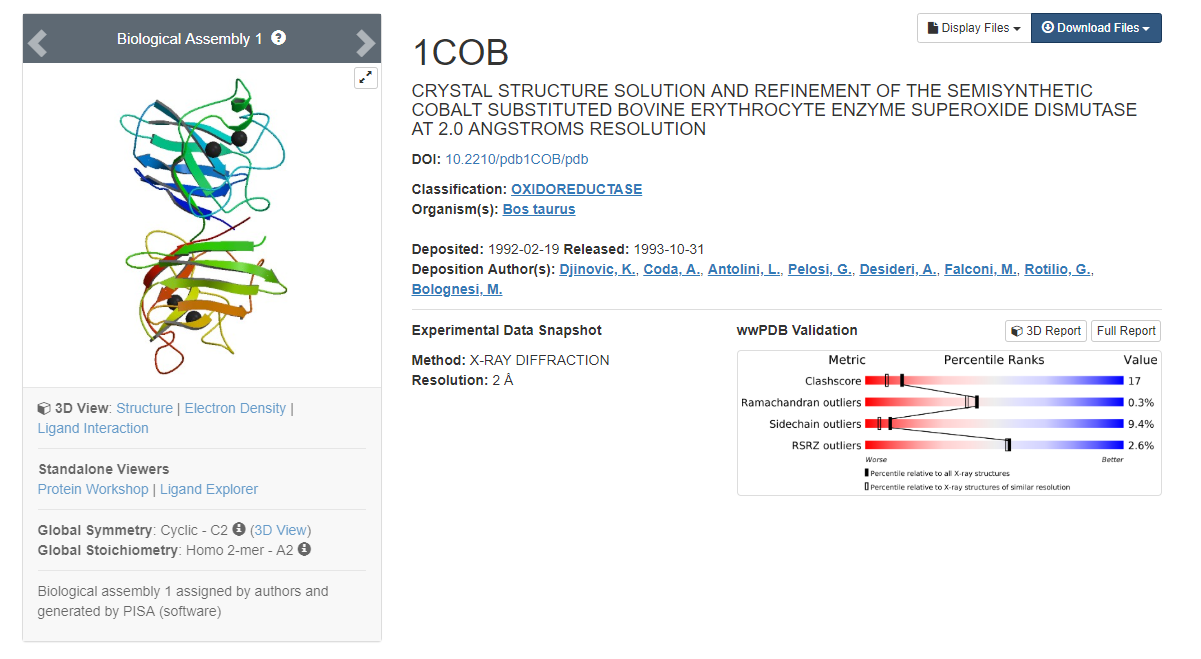
\includegraphics[width=\columnwidth]{clip-pdb.png}
	\end{subfigure}
\end{figure}
%
\begin{figure}[H]\ContinuedFloat
	\centering
	\begin{subfigure}[h]{\columnwidth}
		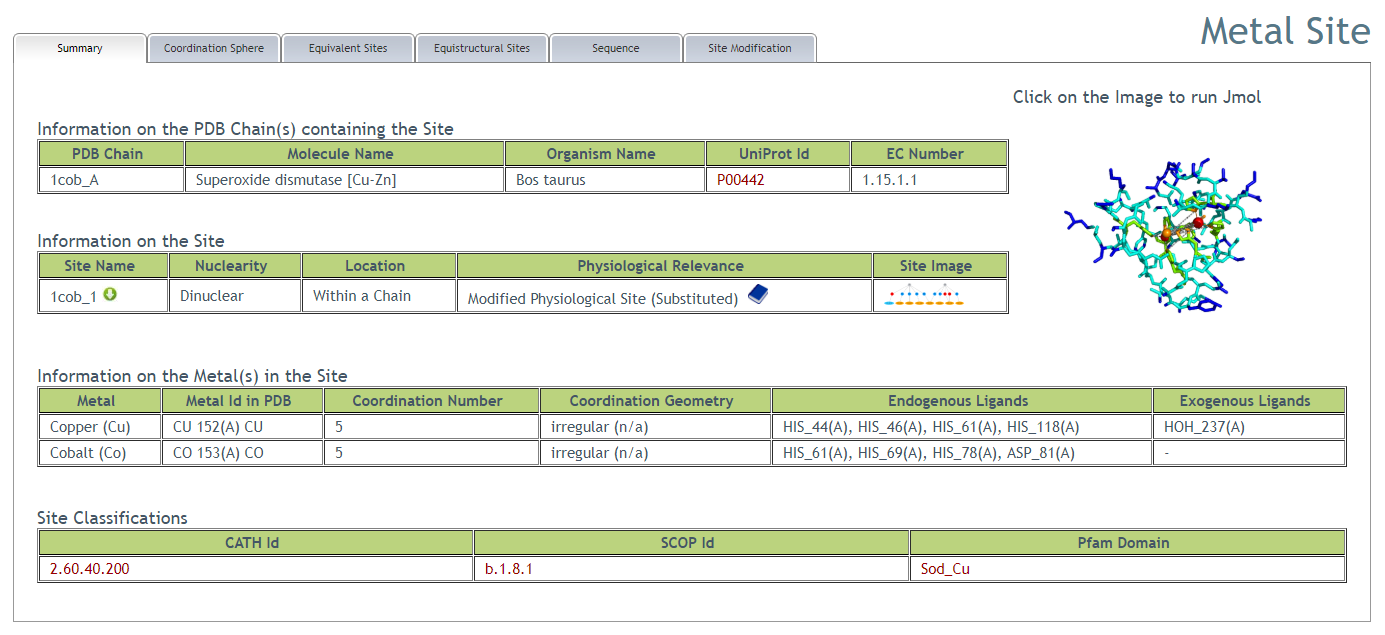
\includegraphics[width=\columnwidth]{clip-metalpdb.png}
	\end{subfigure}
	\caption[Overview of protein database resources]
	{
		\textbf{Overview of protein database resources}.
		The Protein Data Bank (PDB) contains all published protein crystal structures and downloadable files. File formats are text readable .mmCIF or .pdb formats which contain experimental metadata and atomic locations. The metal PDB (\mPDB{}) only contain entries with metal ligands. Entires also provide additional data derived from the PDB files such as metal location, metal site environment, and metadata of the protein origin using other database servers such as Uniprot and Pfam.
	}
	\label{\figname{C}{1}}
\end{figure}

The goal is to somehow reorganize the 3-dimensional information of each protein structure into a processable dataset for statistical analysis. Once an adequate dataset is derived, the next step would be to apply statistical or machine learning framework to discover patterns between metals and their preferred (or most occuring) protein-binding environment. It may not be necessary to deconstruct the entire protein structure, but to only analyze the vicinity around the metal binding site. Within these binding sites, assumptions around the relevance of each parameter (i.e. features) can be made, such as the importance of the distances between amino acids, identity of the amino acid, types of bonding, bonding geometry, and so on. With the appropriate machine learning tools it may be possible to train a model to understand these features and how it may impact metal binding affinity. The potential results can help answer two specific questions: 1) given an unknown binding site, how likely is it to be a metal binder, and if so, which metal? and 2) given a desired metal, what is the optimal sequence and arrangement of amino acids that confer the greated binding affinity?

%===========================================================================%
% Methods
%===========================================================================%
\section{Methods, algorithms, \& data processing}
The interface between biological data and designing an analytical pipeline to consume, transform, and interpret such data is possibly one of the most difficult steps in bioinformatics. The question arises as to how biological data, which is typically unordered, noisy, and sometimes uninterpretable by both machine and human, can be extracted of its fundamental features and then analyzed as a sequence of numbers or categories. Throughout these transformations, a caution is to maintain as much biological relevance without introducing contrived data that is not present in the original dataset, or eliminating/ignoring relevant data for the sake of efficiency or simplicity.

%-----------------------------------------------------------------%
% SUBSECTION
%-----------------------------------------------------------------%
\subsection{Extracting data from the metal PDB}
List of protein structures with metal ligands was extracted from the \mPDB{} by automating a webscraper that fetched all protein files that contained either Ag, Al, Au, Ba, Ca, Cd, Co, Cr, Cs, Cu, Fe, Ga, Hg, In, K, Li, Mg, Mn, Na, Ni, Pb, Pd, Pt, Rb, Sr, W, and Zn (there were no files that containted As, Si)\footnote{
	Rare earth metals for Ce, Er, Eu, Gd, Ho, La, Lu, Os, Pa, Pr, Re, Sm, Ta, Tb, U, Yb were also extracted but not used in this analysis.
}.

The data for each file contained a PDB ID (a unique 4 digit alphanumeric code representing the protein structure), a number next to the PDB ID representing the metal instance (one protein can contain multiple metal binding sites, hence suffixing the ID code with incrementing numbers);
the metal or metals found in that binding pocket;
a string denoting the molecule which the metal belongs to (often it is just the metal, but for example a heme group would be included because of its Fe center) the numeric location of the metal (all atoms and molecules in a PDB file format are numbered), the chain letter, and the metal identity;
and finally the ligands determined by the \mPDB{} to be significant binding partners. These metal binding partners were delimited by a 3 amino acid or molecular code, followed by the numeric location of the binding partner, followed by a chain letter in which the binding partner was part of in the overall protein structure. The data structure for the raw data taken from the \mPDB{} can be found in \TABLE~\ref{\inputtable{C}{1}}.

%~~~~~~~~~~~~~~~~~%
% Table - raw data
%~~~~~~~~~~~~~~~~~%
\begin{table}[H]
\footnotesize
\centering
	\begin{tabular}{lllL{5cm}L{2.5cm}}
  \toprule
  & SiteName & Metal(s) & Metal(s) in pdb file & Ligand(s) \\
  \midrule
  \textit{format}
    & PDBID\_no.
    & metal\textsubscript{x}
    & molecule\_loc(chain)\_metal
    & residue\_loc(chain)\\
  \textit{example}
    & 1apq\_2
    & Cu
    & CU\_125(A)\_CU
    & TYR\_76(A), HIS\_105(A) \\
  \textit{example}
    & 1arm\_1 & Hg, Cu
    & CU\_315(A)\_CU
    & GLU\_270(A), HOH\_320(A) \\
    & &
    & HG\_310(A)\_HG
    & HIS\_69(A), GLU\_72(A), HIS\_196(A), TRS\_319(A), HOH\_320(A) \\
  \bottomrule
\end{tabular}

	\caption[Data format of protein files from the \mPDB{}]
	{
		\textbf{Data format of protein files from the \mPDB{}}.
		Data from the \mPDB{} of each metal instance contained the PDB ID, the identity of the metal for that instance, the molecular location of that metal, and the molecular location of the ligands that bind to that metal.
	}
	\label{\inputtable{C}{1}}
\end{table}

%-----------------------------------------------------------------%
% SUBSECTION
%-----------------------------------------------------------------%
\subsection{Filtering and cleaning data}
\label{subsection:appendixC:filter-clean}
Although the data from the \mPDB{} contained valuable information, it does contain missing entries, redundancies, and is of a format which is difficult to parse for basic analytical pipelines that expect numerical values or consistent categorical strings. Therefore, a filtering step was performed to remove any erroneous entries, and the data was transformed to fit a particular format more amenable for downstream analysis (\FIGURE~\ref{\figname{C}{2}}). \mPDB{} entries were further validated by ping'ing the original PDB database to double check the existance of the protein structure.

The first filter was to remove any entries with multiple metals per metal binding site, as this would confuse the analysis as to which metal was more significant in the metal binding pocket. The second filter was whether or not the PDB file exists. Unfortunately some PDB files were either removed, archived, or did not exist when checked on \url{https://www.rcsb.org/}. The third filter was whether or not the metal PDB data contained valid annotations of where the metal resides, both in the chain lettering and metal numbering. In some cases, some annotations in the \mPDB{} were incorrect, and some metals did not exist in a small fraction of provided protein structures.

During the filtering and cleaning step, more features were extracted from the \mPDB{} and PDB database. Useful features such as metal valency, metal binding geometry, the geometry quality (distorted or regular) were extracted. Additional metadata was extracted to paint a better picture of the protein (although not necesary for the analytical framework) such as UNIPROT ID, organism, and enzyme commission annotations (example of the new dataset structure is tabulated in \TABLE~\ref{\inputtable{C}{2}}).

%=======================%
% FIGURE - data pipeline
%=======================%
\begin{figure}[H]
  \centering
  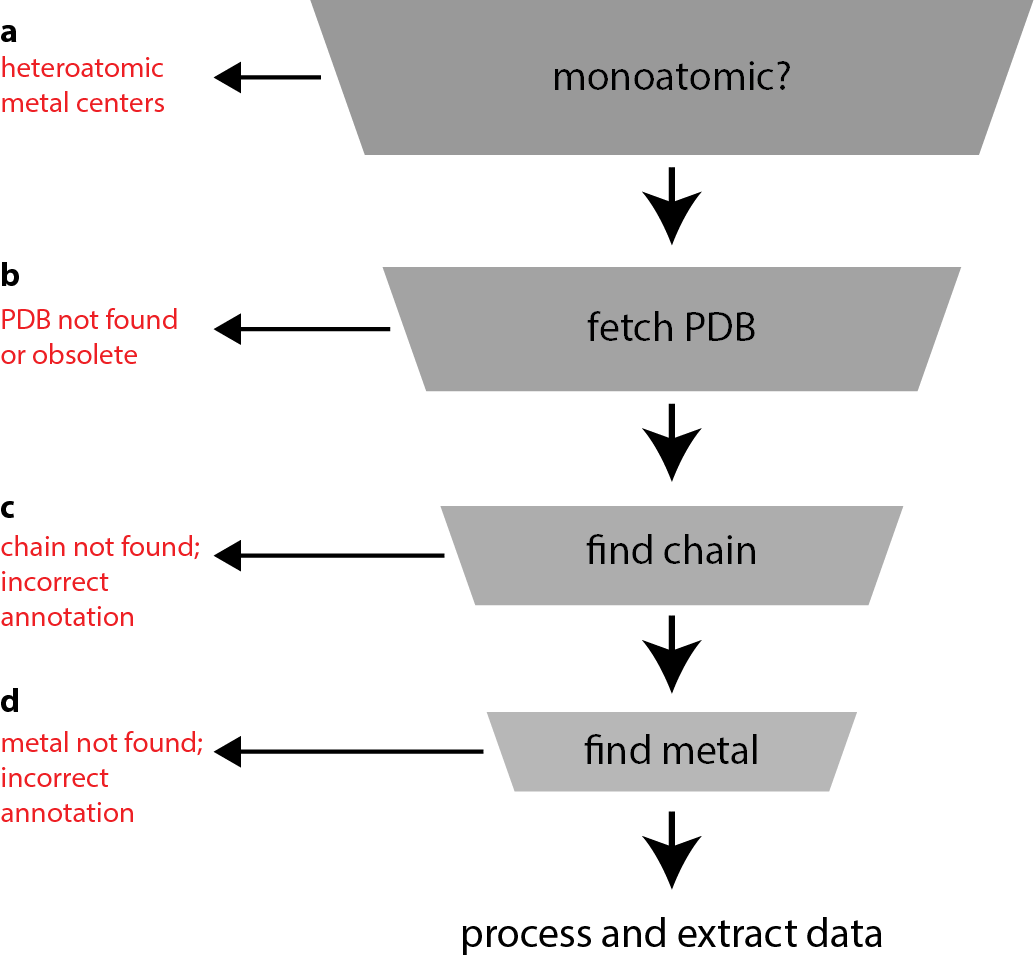
\includegraphics[width=0.5\columnwidth]{data-pipeline.png}
  \caption[Pipeline for parsing and extracting PDB information from the metal PDB]
  {
    \textbf{Pipeline for parsing and extracting PDB information from the metal PDB}.
    (\textbf{a}) Entries that contained multiple metal atoms per metal site were removed to avoid confusion during analysis.
    (\textbf{b}) PDB files that were unfetchable (e.g. obsolete, archived, or non-existent) were ignored.
    (\textbf{c, d}) Annotations provided by the metal PDB were sometimes incorrect. Often this would occur with wrong chain numberings or non-existent metal locations. This filtering step was performed after retrieving the protein structure from the PDB (\url{https://www.rcsb.org/}).
  }
  \label{\figname{C}{2}}
\end{figure}
\clearpage % force page break for following table

%~~~~~~~~~~~~~~~~~~~%
% Table - clean data
%~~~~~~~~~~~~~~~~~~~%
\begin{table}[H]
\centering
	% part 1
	\begin{subtable}[H]{\columnwidth}
		\caption{}
		\centering
		\footnotesize
		\begin{tabular}{llllll}
  \toprule
  & ID & instance & chain & location id & metal id \\
  \midrule
  \textit{format} & PDBID & metal number & A, B, \ldots & loc(chain) & metal atom location \\
  \textit{example} & 1q06 & 1 & B & 300(B) & 24985 \\
  \bottomrule
\end{tabular}

	\end{subtable}
\end{table}
%
\vspace{-\baselineskip}
%
\begin{table}[H]
\ContinuedFloat
	% part 2
	\begin{subtable}[H]{\columnwidth}
		\caption{}
		\centering
		\footnotesize
		\begin{tabular}{lL{3cm}L{3cm}L{2cm}L{1.8cm}}
  \toprule
  & protein & organism & Uniprot & EC \\
  \midrule
  \textit{format} & UNIPROT protein name & UNIPROT protein name & Uniprot accession number & enzyme commission number \\
  \textit{example} & HTH-type transcriptional regulator CueR & Escherichia coli & P0A9G4 & - \\
  \bottomrule
\end{tabular}

	\end{subtable}
	% part 3
	\begin{subtable}[H]{\columnwidth}
		\caption{}
		\centering
		\footnotesize
		\begin{tabular}{lllll}
  \toprule
  & valency & geometry & idealized & ligands \\
  \midrule
  \textit{format} & 0--9 & linear, trigonal, \ldots & -, distored, regular & residue\_loc(chain) \\
  \textit{example} & 2 & linear & regular & CYS\_112(B), \ldots \\ % CYS\_120(B) \\
  \bottomrule
\end{tabular}

	\end{subtable}
	\caption[Tranformed dataset structure of protein entires filtered from the \mPDB{}]
	{
		\textbf{Tranformed dataset structure of protein entires filtered from the \mPDB{}}.
		(\textbf{a}) The original metal PDB entries were cleaned to individully represent the PDB ID, metal instance for that PDB file, chain location, molecular location of the metal, and atomic location of the metal.
		(\textbf{b}) Additional metadata was extracted such as the UNIPROT ID, organism name, accession number, etc.
		(\textbf{c}) Categorical data such as metal valency, metal binding geometry, and ligands were also taken from the metal PDB.
	}
	\label{\inputtable{C}{2}}
\end{table}

%-----------------------------------------------------------------%
% SUBSECTION
%-----------------------------------------------------------------%
\subsection{Creating datasets processable by machine learning algorithms}
The filtered and cleaned data from the \mPDB{} had yet to undergo another transformation in order to be inputted into a statistical or machine learning framework. To create such an input--output pipeline the data structure was converted to numerical or categorical features. More so, the previously processed features were not feature rich (\TABLE~\ref{\inputtable{C}{2}}), as in, they did not quantitatively explain the metal-protein structure relationship in detail. An example would be the sparse 1--5 amino acid binding partner description per metal coordination sphere. Therefore, a new algorithm was developed to extract 3-dimensional data from the protein crystal structure which bared more fine-grained atomic data. The algorithm developed was a variation of the nearest-neighbor algorithm~\cite{arya1998optimal} in which an imaginary radii stretched from the metal center is modelled to extract the closest molecule/amino acid from that metal center (\FIGURE~\ref{\figname{C}{3}}). The discovered neighbors were further processed to determine which atom from that molecule were closest, and the distance between the atom and the molecule from the metal center were also calculated\footnote{
	Bio.PDB package in python was used to handle PDB structural data: \url{https://biopython.org/wiki/The_Biopython_Structural_Bioinformatics_FAQ}
}.

%====================%
% Figure - algorithm
%====================%
\begin{figure}[H]
	\centering
	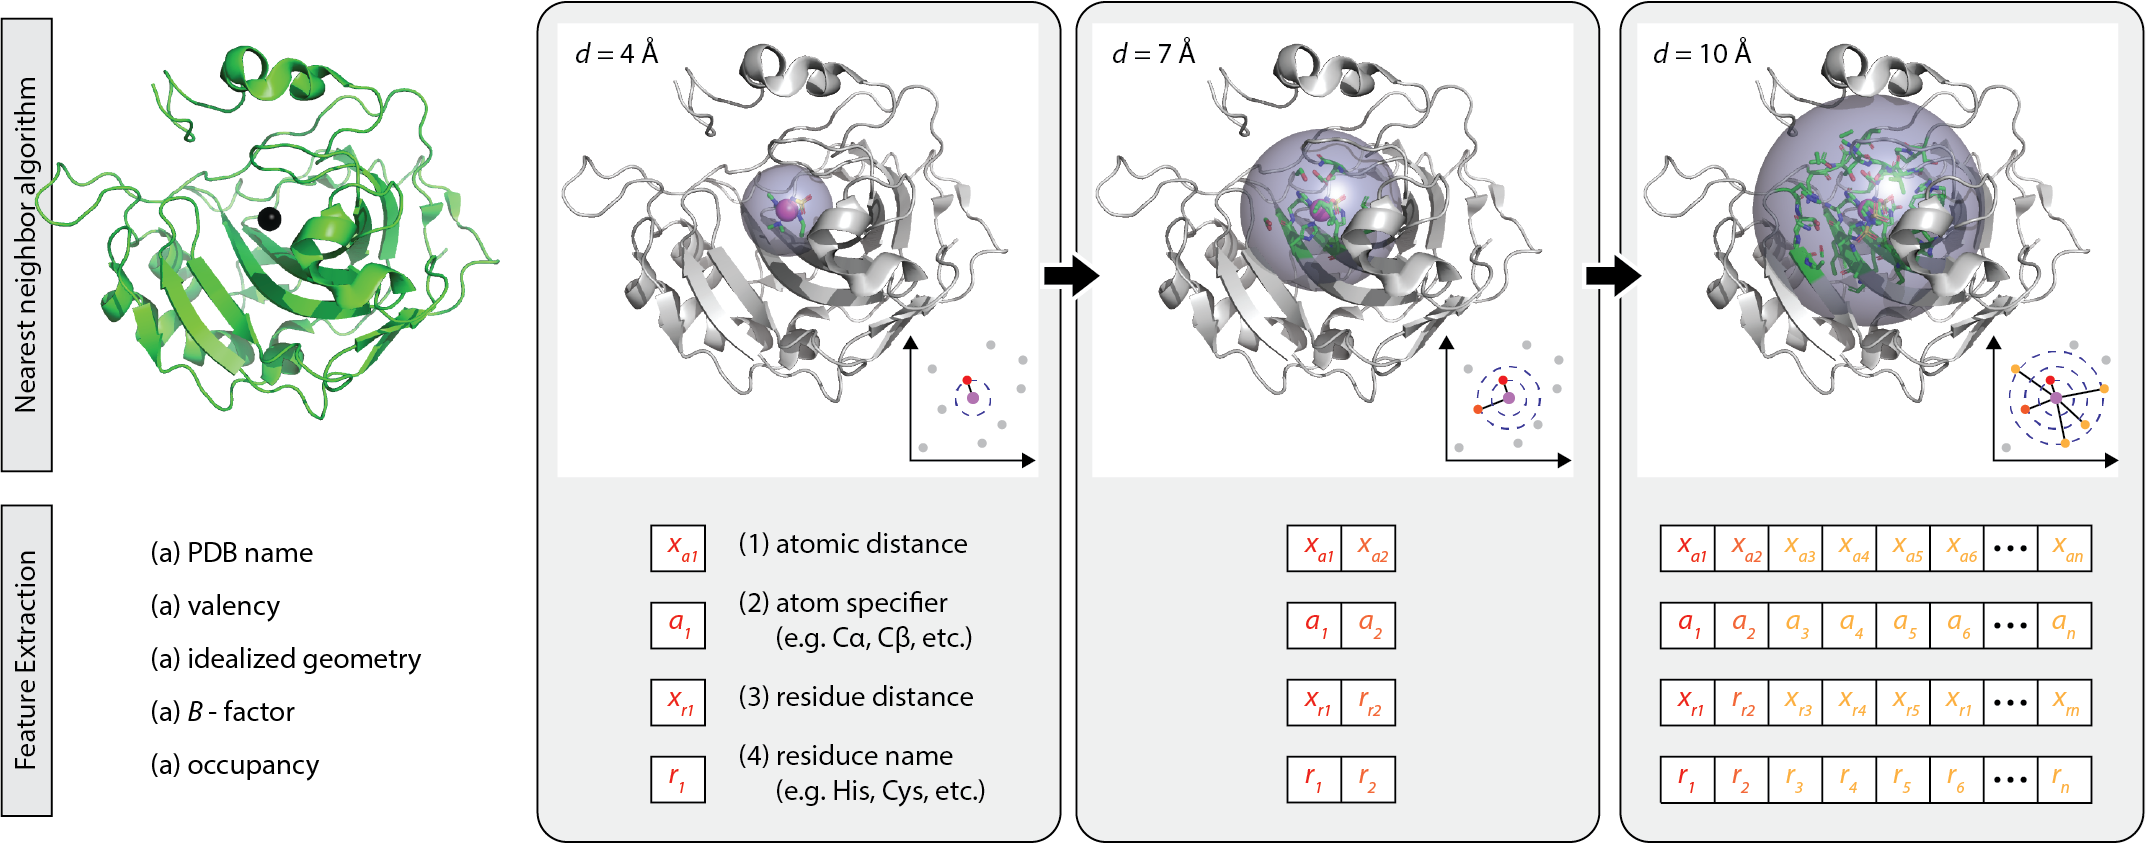
\includegraphics[width=\columnwidth]{schematic.png}
	\caption[Variation of the nearest-neighbor algorithm to extract molecular and atomic neighbors from the metal center of a protein structure]
	{
		\textbf{Variation of the nearest-neighbor algorithm to extract molecular and atomic neighbors from the metal center of a protein structure}.
		Molecular and atomic neighbors at incremental radii away from the metal center were identified using the nearest-neighbor algorithm and stored in arrays. These arrays were later concatenated to create either a 2D dataset or 1D row of features. Additional parameters were extracted during the algorithm. These parameters were the valency and geometry of the metal-binding environment, the metal's $\beta$-factor and its percent occupancy.
	}
	\label{\figname{C}{3}}
\end{figure}

The features collected were the atoms closest to the metal center, and their distances away from the metal center. The same process was performed for nearest neighbor molecules and their distances. These features were ordered from closest to furthest, the closest being 1 \AA{} and furthest being 50 \AA{} away. All features were concatenated to create a 1D aray with each analyzed protein structure representing a row of a larger 2-dimensional data structure. These datasets were segregated by metal's analyzed. For example, there existsed separate datasets of acquired nearest-neighbor information for Li, Na\ldots{}Pb, where each for of each dataset represents the features extracted from a single protein structure.

In addition, several metadata parameters were included in the feature list. They were the metal's $\beta$-factor and percent occupancy. These values helped score the confidence of the metal location in the protein structure, and future work would use these values to under-weigh or ignore potential outliers or bad instances.

%~~~~~~~~~~~~~~~~~~~~~~%
% Table - analysis data
%~~~~~~~~~~~~~~~~~~~~~~%
\begin{table}[H]
	% part 1
	\begin{subtable}[H]{\columnwidth}
		\caption{}
		\centering
		\footnotesize
		\begin{tabular}{lllclllcc}
  \toprule
  & metal & ID & valency & geometry & idealized & $\beta$factor & occupancy & anisotropy \\
  \midrule
  \textit{example} & Ag & 1q06 & 2 & linear & regular & 26.6 & 1 & -1 \\
  \bottomrule
\end{tabular}

	\end{subtable}
	% part 2
	\begin{subtable}[H]{\columnwidth}
		\caption{}
		\footnotesize
		\begin{tabular}{lL{2cm}L{3cm}L{3cm}L{3.5cm}}
  \toprule
  & atom name & atom distance (\AA) & molecule name & molecule distance (\AA)\\
  \midrule
  \textit{example}
    & SG, CB, CB, CB, CA, O
    & 2.35, 3.2, 3.37, 3.5, 3.51, 3.6
    & CYS, CYS, CYS, SER, CYS, SER
    & 4.17, 3.51, 4.17, 3.88, 3.51, 3.88 \\
  \bottomrule
\end{tabular}

	\end{subtable}
	\caption[Training set data structure as input to machine learning frameworks]
	{
		\textbf{Training set data structure as input to machine learning frameworks}.
		(\textbf{a}) Several metal-protein specific parameters such as the metal's valency and geometry, as well as its $\beta$-factor and percent occupancy were collected.
		(\textbf{b}) Arrays of atom names, atom distances, residue names, and residue distances sorted from closet to furthest from the metal center were concatenated into a single array.
	}
	\label{\inputtable{C}{3}}
\end{table}

%===========================================================================%
% Results
%===========================================================================%
\section{Results}

%-----------------------------------------------------------------%
% SUBSECTION
%-----------------------------------------------------------------%
\subsection{Analysis of protein-metal data curated by the \mPDB{}}
A significant portion of the curated protein structures from the \mPDB{} were not usable, primarily because there were multiple metals per metal binding site, and some of the chain and metal location annotations were incorrect. For metals that had more than 10 PDB entires, the filtering step removed almost 25--40\% of entires (\FIGURE~\ref{\figname{C}{4}}a).

The metals with the most PDB entries were Na, Mg, Ca, and Zn. However, alkaline and alkaline-earth metals like Na and Mg may be over-represented because these metals are frequently present in buffers during crystallization.More so, during PDB submission man of the crystal structure solute environment remains annotated, scoring hundreds to thousands of spectator ions. Unfortunately, the \mPDB{} does not filter these entries, and in this work these entries propogated through the analysis. To remove these false-positive metal-bound proteins would require differentiating metals in the buffer from metals bound to the protein. To do so would require accessing the PDB structure directly and querying every metal. Alternatively, a threshold could be set that if a protein contains more than X number of metals, specifically Na, Mg, etc., then it should be eliminated. However, this assumption is crude, and may falsely eliminate good protein structures.

The fact that many metals in the protein structure entries were solutes rather than bound metals help explains the high $\beta$-factors and low percent occupancy for most of the alkaline and alkaline-earth metals. Also, many metals which are rarely found in proteins such as the metalloid and noble metals like Pt and Hg had poor $\beta$-factors and percent occupancies (\FIGURE~\ref{\figname{C}{4}}b). When looking at the metal-bound protein structures holistically, on average each structure contains 2 or less binding sites (\FIGURE~\ref{\figname{C}{4}}c). In other words, it is likely that a protein structure containing a particular metal will have one or two binding pockets for that metal.

%======================%
% number of files chart
%======================%
\begin{figure}[H]
	\begin{subfigure}{\columnwidth}
		\centering
		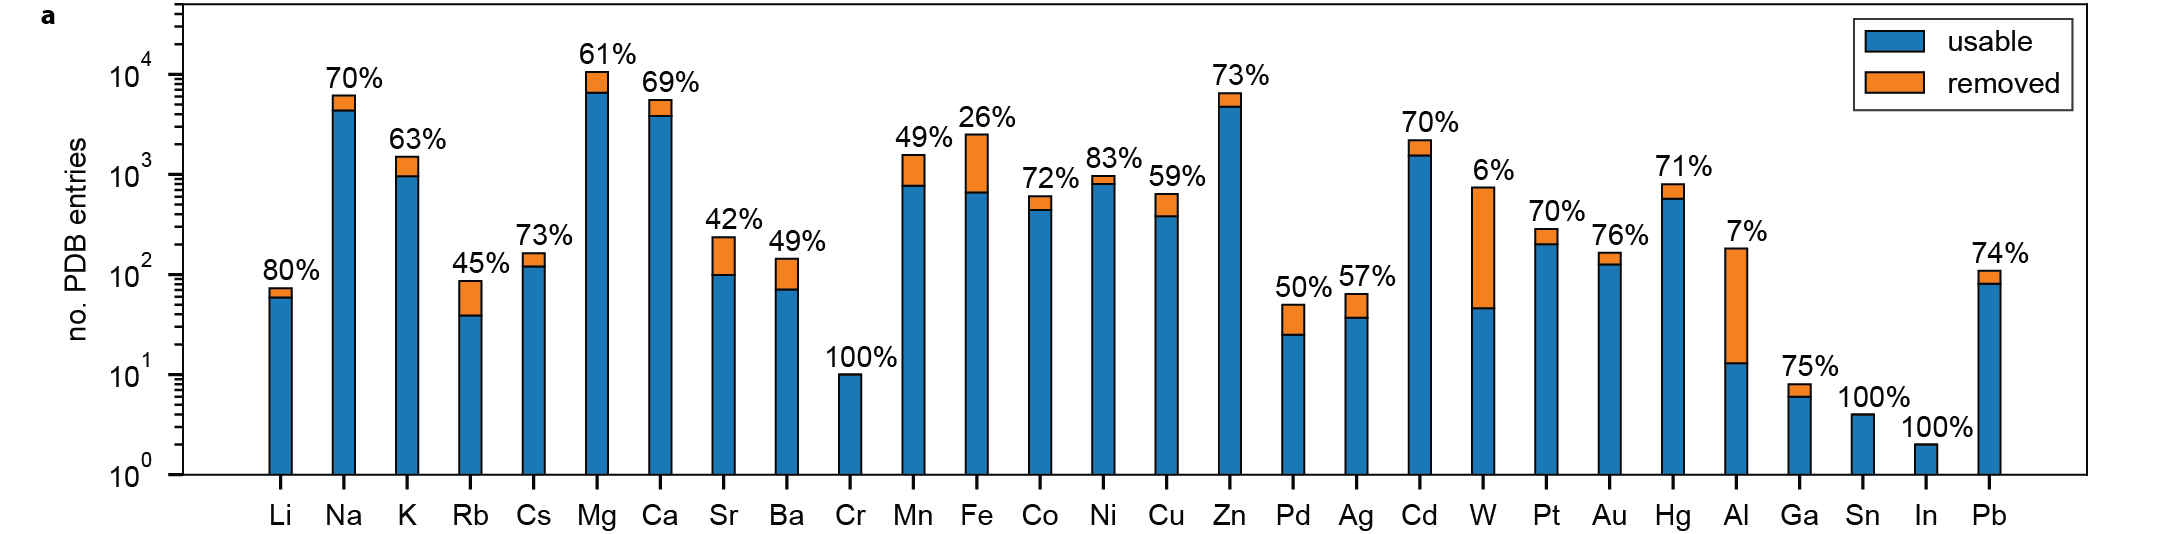
\includegraphics[width=\columnwidth]{initial-stats_a.png}
	\end{subfigure}
\end{figure}
%
\begin{figure}[H]\ContinuedFloat
	\begin{subfigure}{\columnwidth}
		\centering
		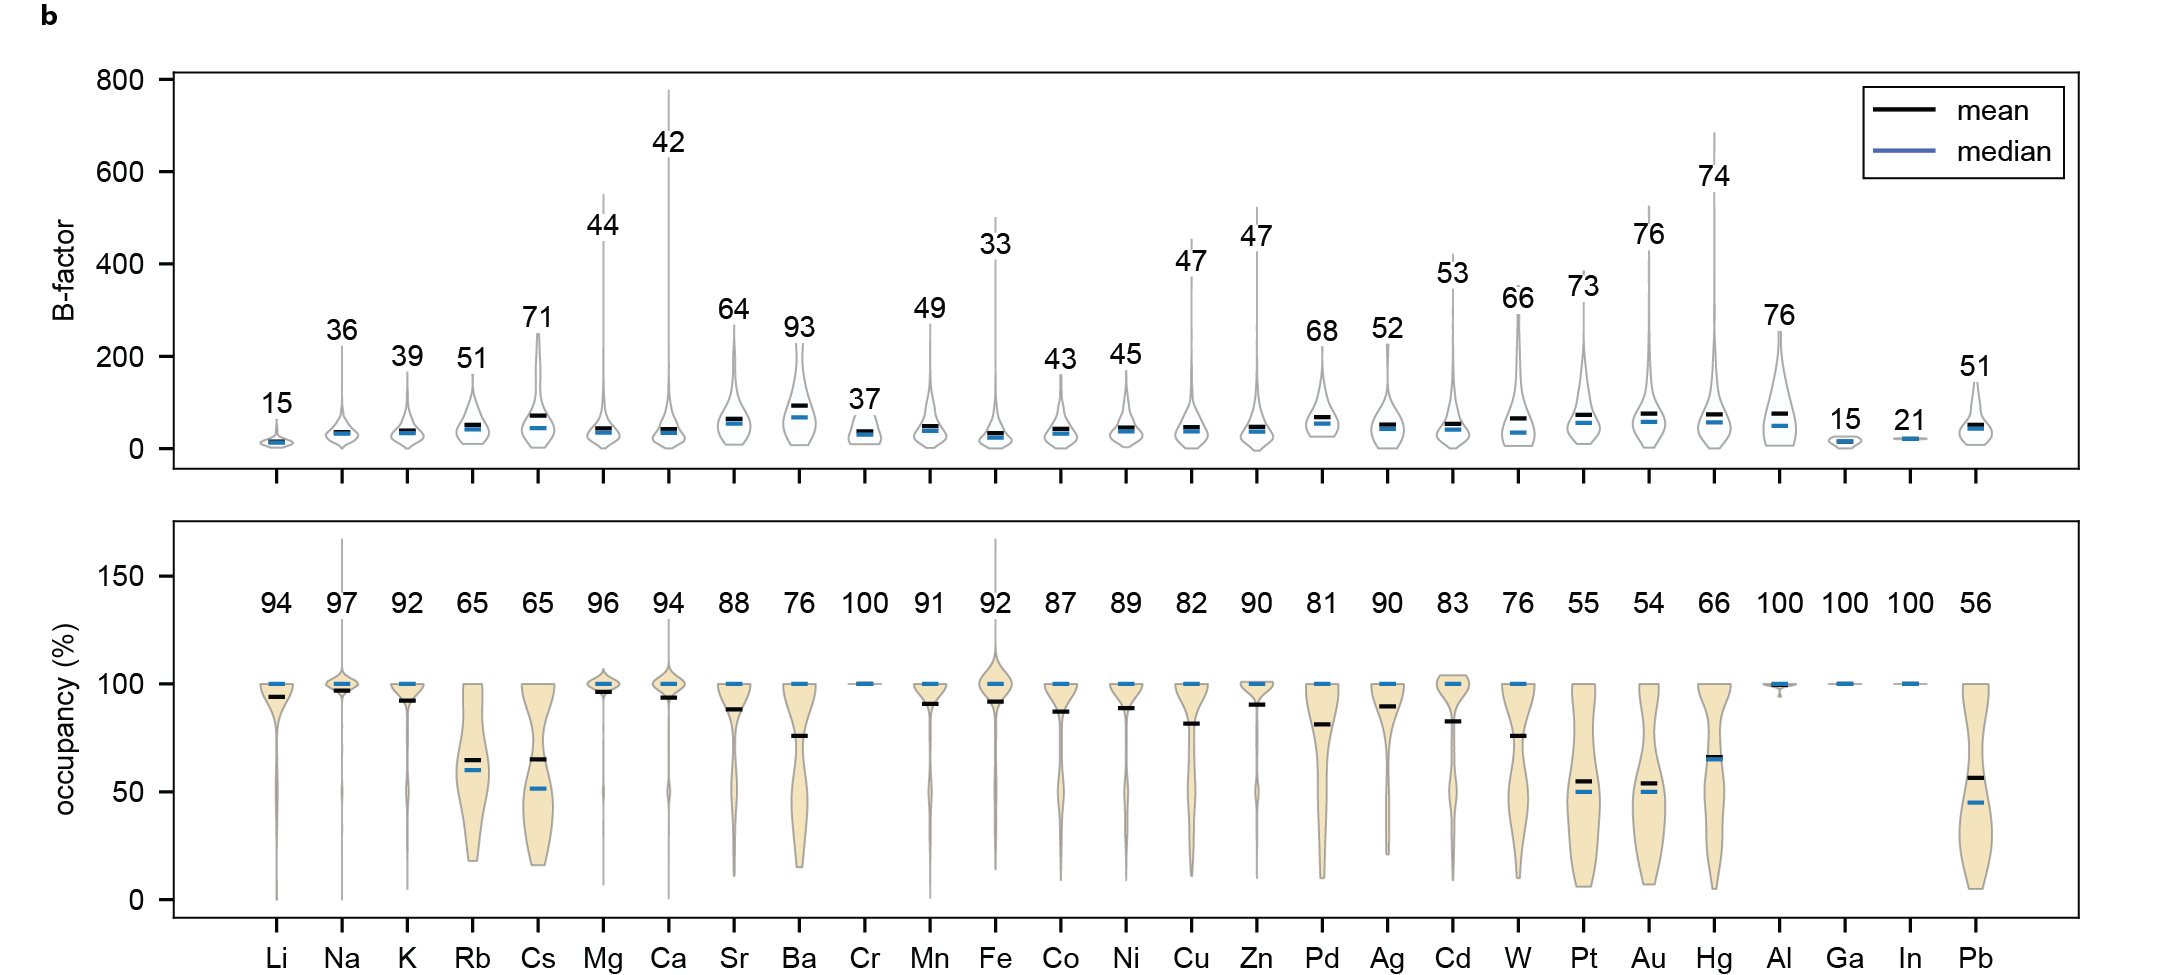
\includegraphics[width=\columnwidth]{initial-stats_b.png}
	\end{subfigure}
\end{figure}
%
\begin{figure}[H]\ContinuedFloat
	\begin{subfigure}{\columnwidth}
		\centering
		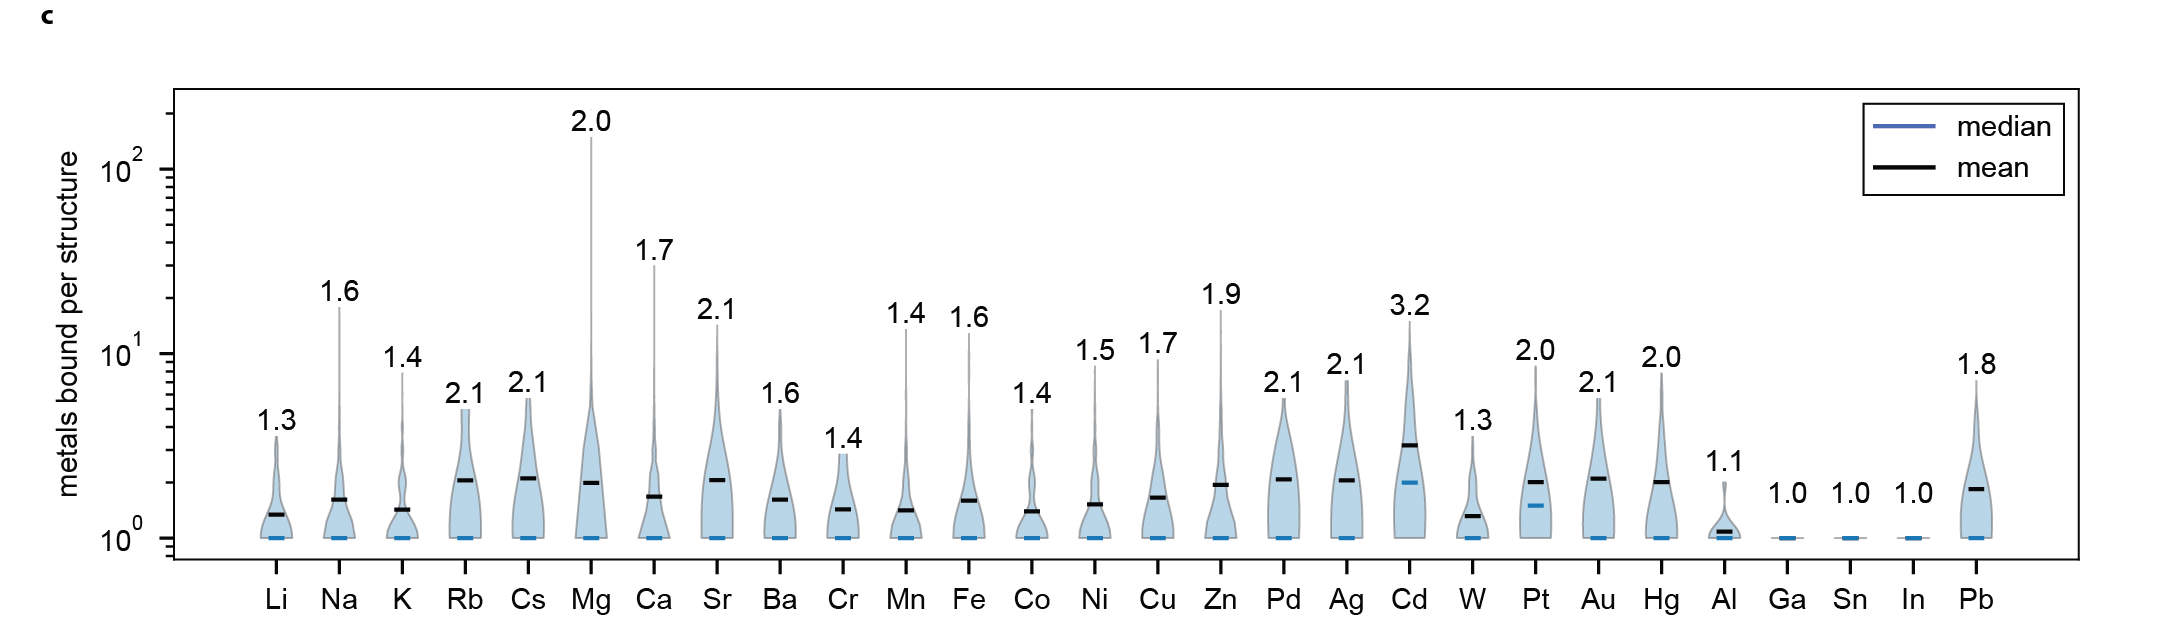
\includegraphics[width=\columnwidth]{initial-stats_c.png}
	\end{subfigure}
% \end{figure}
%
% \begin{figure}[H]\ContinuedFloat
	\caption[Number of usable metal PDB entries and their statistics]
	{
		\textbf{Number of usable metal PDB entries and their statistics}.
		(\textbf{a}) Several protein structures provided by the \mPDB{} were not usable and had to be filtered (see \FIGURE~\ref{\figname{C}{2}} on filtering criteria). Note the y-axis is in log scale, and that bar heights are not linearly proportional. Some metals such as Ga, Sn, and In, particularly from the semi-metals contained very few entries (less than 10). Alkaline and alkaline-earth metals were highly represented, most likely because these metals are often present as dissolved solutes during protein crystallization.
		(\textbf{b}) Plot showing $\beta$-factors and percent occupancy of each metal. Low $\beta$-factors suggest more accurate metal position, and higher percent occupancy suggest greater confidence in metal localization. Metals that are not often found in proteins such as Rb, Cs, Hg, etc. have high $\beta$-factors and low percent occupancies, which may suggest that these are not natural or favorable binding environments.
		(\textbf{c}) Plot showing the average number of metal binding sites per protein for a given metal. Overall, the average metal-binding proteins usually contain less than 2 metal binding sites.
	}
	\label{\figname{C}{4}}
\end{figure}

In most metal-binding environments many metals, especially the alkaline and alkaline-earth metals, have valencies of 1 or 2. For transition metals they may be found in several valent states ranging from 1--7 because of the electron donating d-orbitals; however, still many transition metal co-factors are found in the divalent state such as \ce{Mn^2+}, \ce{Fe^{2+}}, \ce{Zn^{2+}}  etc. So it was surpising to see that the valencies calculated by the \mPDB{} were not between 1--2, but rather varying dramatically.

%~~~~~~~~~~~~~~~~~~~~%
% table on geometries
%~~~~~~~~~~~~~~~~~~~~%
\begin{table}[H]
\setlength\extrarowheight{-5pt}
\centering
	\resizebox{\columnwidth}{!}{%
		\begin{tabular}{l l l l c c}
	\toprule
	no. & val. & abbrv. & full geometry name	& instances & percent \\
	\midrule
	1   & 0       & -     & -                                                                       & 4086      & 15\%     \\
	2   & 0       & IRR   & irregular                                                               & 7530      & 28\%     \\
	3   & 2       & TRV   & trigonal plane with a vacancy                                           & 2209      & 8\%      \\
	4   & 2       & LIN   & linear                                                                  & 230       & 1\%      \\
	5   & 3       & TRI   & trigonal plane                                                          & 214       & 1\%      \\
	6   & 3       & SPV   & square plane with a vacancy                                             & 634       & 2\%      \\
	7   & 3       & TEV   & tetrahedron with a vacancy                                              & 1047      & 4\%      \\
	8   & 4       & BVP   & trigonal bipyramid with a vacancy (equatorial)                          & 234       & 1\%      \\
	9   & 4       & BVA   & trigonal bipyramid with a vacancy (axial)                               & 505       & 2\%      \\
	10  & 4       & SPL   & square plane                                                            & 537       & 2\%      \\
	11  & 4       & PYV   & square pyramid with a vacancy (equatorial)                              & 1124      & 4\%      \\
	12  & 4       & TET   & tetrahedron                                                             & 1405      & 5\%      \\
	13  & 5       & SPY   & square pyramid                                                          & 1247      & 5\%      \\
	14  & 5       & TBP   & trigonal bipyramid                                                      & 202       & 1\%      \\
	15  & 5       & TPV   & trigonal prism with a vacancy                                           & 87        & 0\%      \\
	16  & 6       & OCT   & octahedron                                                              & 3219      & 12\%     \\
	17  & 6       & TPR   & trigonal prism                                                          & 49        & 0\%      \\
	18  & 6       & PVP   & pentagonal bipyramid with a vacancy (equatorial)                        & 491       & 2\%      \\
	19  & 6       & CTF   & trigonal prism, square-face monocapped with a vacancy (capped face)     & 40        & 0\%      \\
	20  & 6       & CTN   & trigonal prism, square-face monocapped with a vacancy (non-capped edge) & 95        & 0\%      \\
	21  & 6       & PVA   & pentagonal bipyramid with a vacancy (axial)                             & 129       & 0\%      \\
	22  & 6       & CON   & octahedron face monocapped with a vacancy (non-capped face)             & 77        & 0\%      \\
	23  & 6       & COF   & octahedron face monocapped with a vacancy (capped face)                 & 71        & 0\%      \\
	24  & 7       & HVP   & hexagonal bipyramid with a vacancy (equatorial)                         & 49        & 0\%      \\
	25  & 7       & CUV   & cube with a vacancy                                                     & 4         & 0\%      \\
	26  & 7       & CTP   & trigonal prism square-face monocapped                                   & 99        & 0\%      \\
	27  & 7       & PBP   & pentagonal bipyramid                                                    & 544       & 2\%      \\
	28  & 7       & HVA   & hexagonal bipyramid with a vacancy (axial)                              & 2         & 0\%      \\
	29  & 7       & COC   & octahedron face monocapped                                              & 148       & 1\%      \\
	30  & 7       & SAV   & square antiprism with a vacancy                                         & 83        & 0\%      \\
	31  & 8       & BTT   & trigonal prism triangular-face bicapped                                 & 0         & 0\%      \\
	32  & 8       & BOC   & octahedron trans-bicapped                                               & 0         & 0\%      \\
	33  & 8       & BTS   & trigonal prism square-face bicapped                                     & 56        & 0\%      \\
	34  & 8       & SQA   & square antiprism                                                        & 79        & 0\%      \\
	35  & 8       & CUB   & cube                                                                    & 3         & 0\%      \\
	36  & 8       & HBP   & hexagonal bipyramid                                                     & 5         & 0\%      \\
	37  & 9       & CSA   & square antiprism square-face monocapped                                 & 0         & 0\%      \\
	38  & 9       & TTP   & trigonal prism square-face tricapped                                    & 0         & 0\%	   \\
	\bottomrule
\end{tabular}

	}
	\caption[Table of metal binding geometries for all metals examined from the metal PDB]
	{
		\textbf{Table of metal binding geometries for all metals examined from the metal PDB}.
		Many metal geometries could not be identified, or were irregular (>40\%). The most prominent geometries were trigonal planar with a vacancy (valency of 2), and octahedral (valency of 8).
	}
	\label{\inputtable{C}{4}}
\end{table}

\noindent Elements such as Li, Na, and K had valencies above 3, and many of the metalloids had valencies above 4 (\FIGURE~\ref{\figname{C}{5}}a). A hypothesis is that these valencies were calculated indirectly by the number of binding partners found in the protein structure. The number of metal-binders predicted by the \mPDB{} may have simply counted the number of ligands and summed them to generate a valency value (\TABLE~\ref{\inputtable{C}{1}}; ``Ligand(s)'' column).

The overall representation of metal geometries were either irregular (28\%), not identifiable (15\%), octahedral (12\%), or trigonal planar with a vacancy (8\%) (\TABLE~\ref{\inputtable{C}{4}}). What this data suggest is that valency could be a poor identifier to distinguish different types of metal binding environments.

%-----------------------------------------------------------------%
% SUBSECTION
%-----------------------------------------------------------------%
\subsection{Differentiating protein-metal interactions by clustering steric and ligand data}
Data strictly derived from the \mPDB{} were used as input datasets for statistical and clustering analysis. The intention was to use features that were filtered and cleaned (\SECTION~\ref{subsection:appendixC:filter-clean}) from the \mPDB{} to help elucidate patterns that could help differentiate metals and their metal-protein binding interactions from one another. The most basic objective was whether or not the curated data from the \mPDB{} could discern between alkaline, transition, metalloids, and noble metals from one another.

%======================%
% mapping ligands
%======================%
\vspace*{\fill} % push to the bottom of the page
\begin{figure}[H]
	\begin{subfigure}[h]{\textwidth}
		\centering
		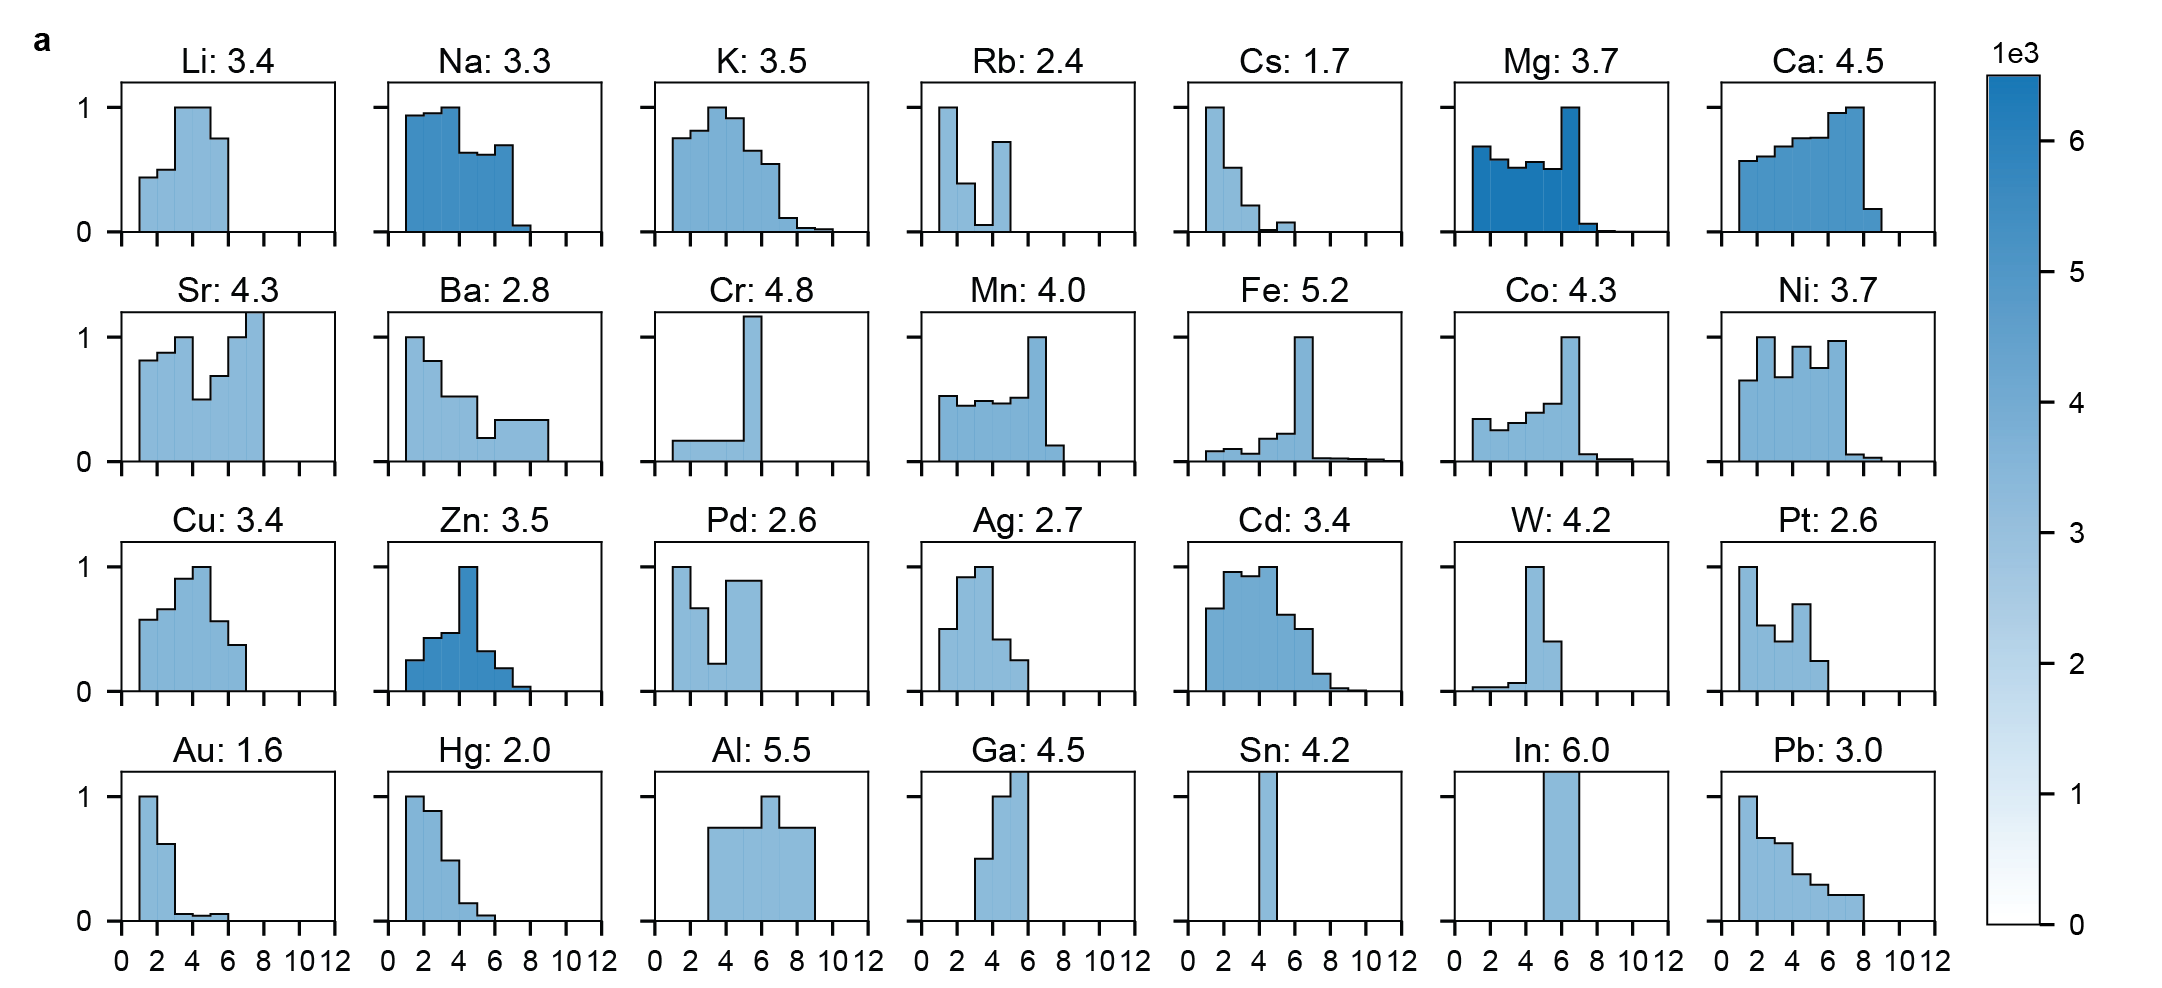
\includegraphics[width=\linewidth]{clustering-valency-a.png}
	\end{subfigure}
\end{figure}
%
\begin{figure}[H]\ContinuedFloat
	\begin{subfigure}[h]{\textwidth}
		\centering
		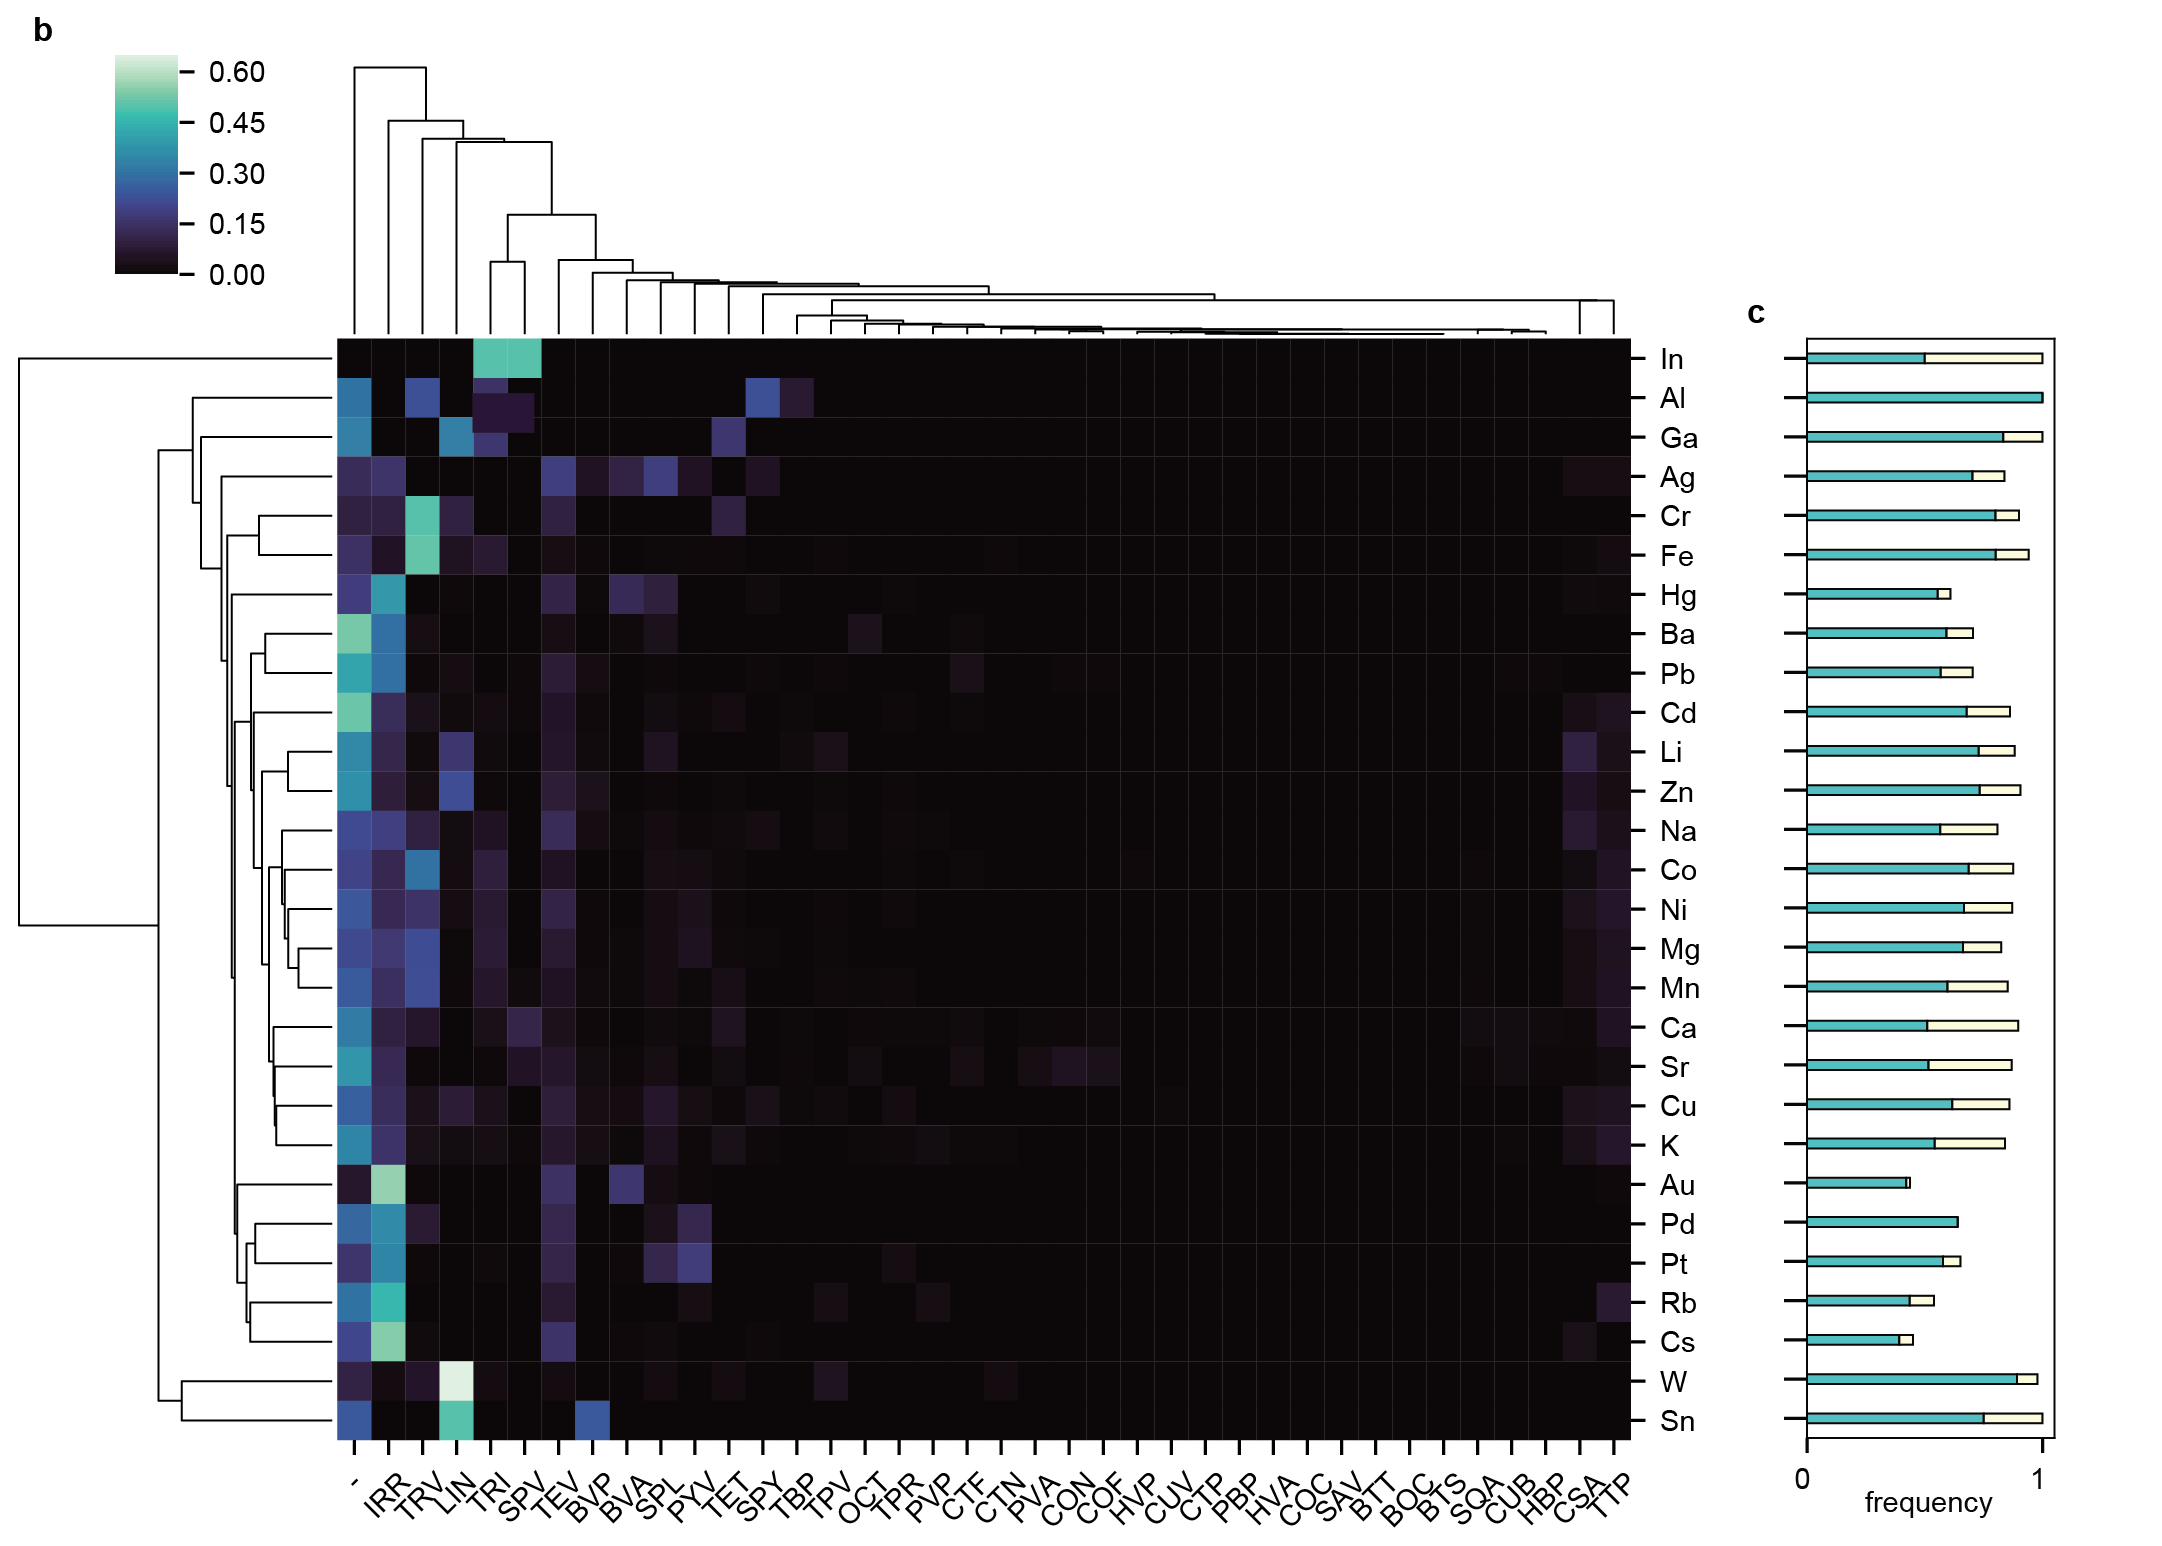
\includegraphics[width=\linewidth]{clustering-valency-b.png}
	\end{subfigure}
	\caption[Analyzing metal valency and geometry data to determine differences between metal groups]
	{
		\textbf{Analyzing metal valency and geometry data to determine differences between metal groups}
		(\textbf{a}) Histogram of valencies for each metal. Typically, most metals found biologically have valencies between 1--2; however, data from the \mPDB{} suggest valencies above 2--, on average3.
		(\textbf{b}) Binned geometry occurances for each metal were clustered to identify any discrimination between metal groups. There were no distinct groupings observed.
		(\textbf{c}) Each geometry was either deemed regular, distorted, or unknown. For each metal, the annotation of each geometry was summed and plotted. The horizontal bar chart represent the frequency of regular (turquoise bar), and frequency of distored (beige bar) for each metal presented in the heatmap b). The remainder up to 1 represents the frequency of unknown.
	}
	\label{\figname{C}{5}}
\end{figure}

Data on the metal's sterics, such as the metal's valency and geometry, were used for clustering analysis. Clusters were generated by using a single linkage method and euclidian distance as the distance metric. Unfortunately, there were no discernable groupings of alkaline metals from transition metals from metalloids, etc. (\FIGURE~\ref{\figname{C}{5}}b). Overall, there was no consistent clustering pattern that could differentiate a metal-protein binding interaction using observations based on the steric environment alone.

Instead of analyzing the metal's sterics, the metal-binding ligands (i.e. amino acid residues) represented in each \mPDB{} entry (\TABLE~\ref{\inputtable{C}{1}} were used instead for clustering analysis. Although the ligand data lacked statistical power (many residue entries were zero), the clustering did show discrimination between certain metal groups (\FIGURE~\ref{\figname{C}{5}}). In particular, the majority of alkaline and alkaline-earth metals were clustered together, and some of the transition, metalloid, and noble metals were segregated with statistical significance.

These preliminary findings suggest that it may be possible to systematically differentiate metals based on their amino acid-binding environment. Simply, a straightforward counting and binning of nearby binding residues was enough to superficially differentiate metals based on their periodic grouping (\FIGURE~\ref{\figname{C}{6}}). To further this investigation, the data provided by the \mPDB{} could be more feature rich if counts of neighboring residues in the metal binding environment were accounted for at varing distances away from the metal, and the same goes for nearby atoms. From here it would be possible to either construct a supervised or unsupervised machine learning model to predict the most common amino acid configuration away from the metal. With these models it may be possible to eventually develop autoencoders or generative models~\cite{goodfellow2014generative} to create de-novo metal-protein binding sites given robust predictions of the metal's nearest-neighbor data.
\clearpage % force page break for following figure

%===================%
% ligand clustering
%===================%
\begin{figure}[H]
	\centering
	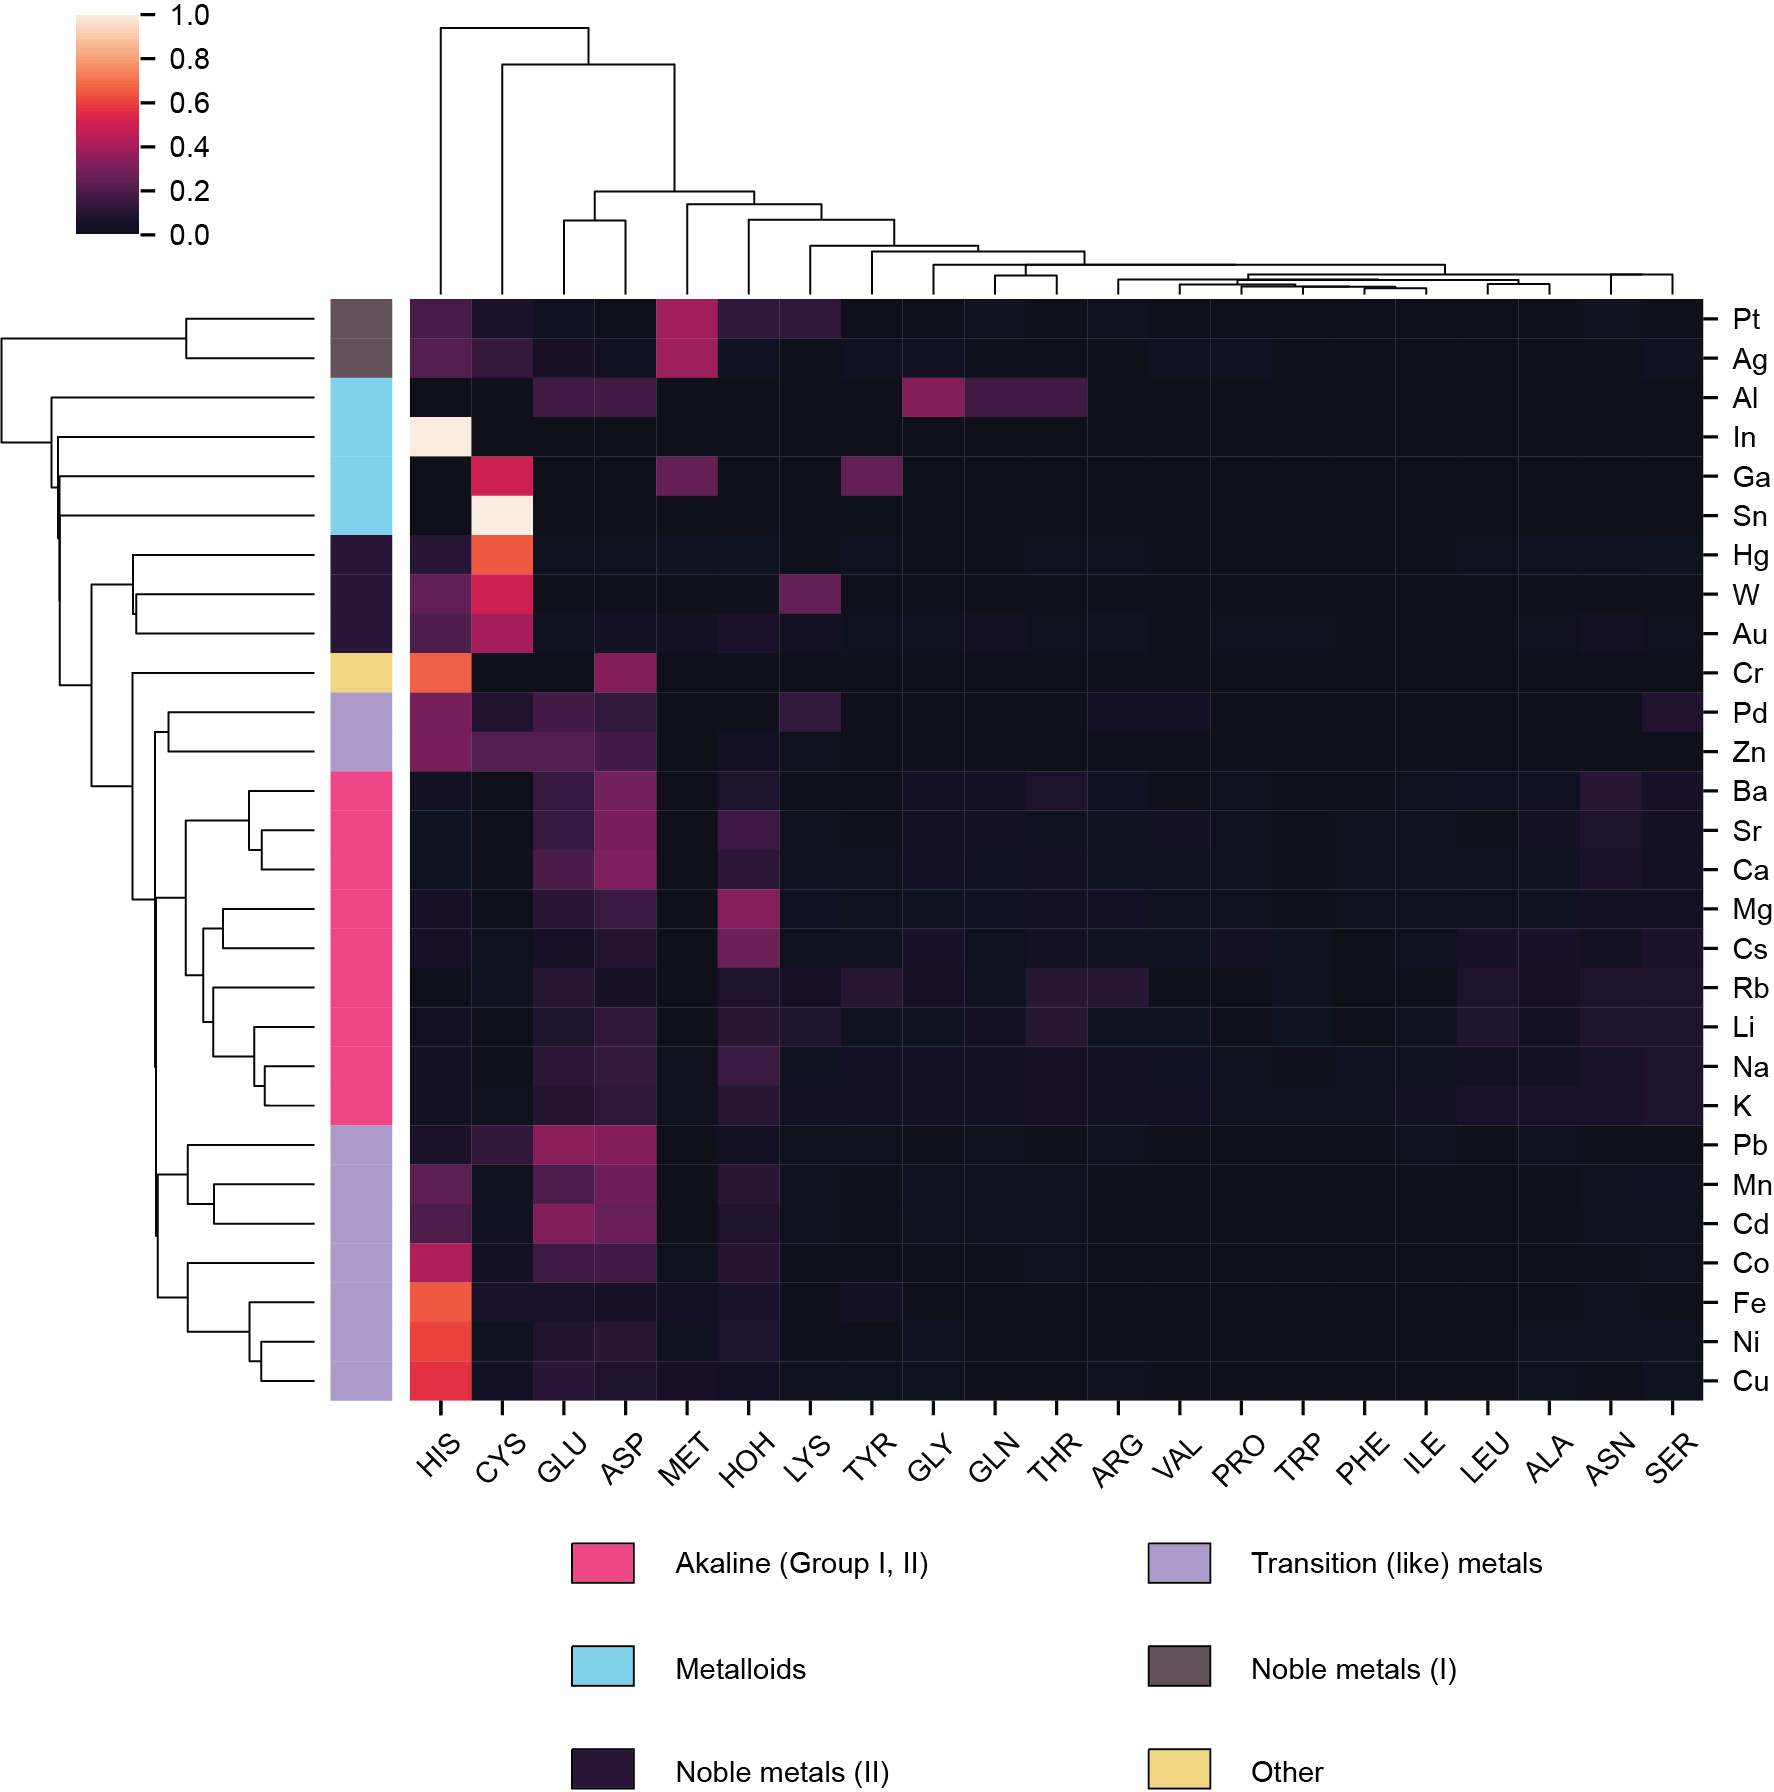
\includegraphics[width=\linewidth]{clustering-ligand-counts.png}
	\caption[Clustering metals based on their metal-binding ligands given data from the \mPDB{}]
	{
		\textbf{Clustering metals based on their metal-binding ligands given data from the \mPDB{}}.
		Alkaline and alkaline-earth metals clustered together (pink rows), whereas some of the transition metals (light purple rows) were separate from the metalloid (turquoise rows) and noble metals (dark pink and brown rows).
	}
	\label{\figname{C}{6}}
\end{figure}
\clearpage % force page break for new section

%~~~~~~~~~~~~~~~~~~~%
% ligand table 1 & 2
%~~~~~~~~~~~~~~~~~~~%
% \begin{table}[H]
% \setlength\extrarowheight{-2pt}
% 	\centering
% 	\resizebox{\columnwidth}{!}{%
% 		\begin{tabular}{llllllllllllllllllllll}
	\toprule
	& HIS  & CYS  & GLU  & ASP  & MET  & HOH  & GLN  & ASN  & THR  & SER  & LYS  & ARG  & GLY  & PRO  & TRP  & TYR  & PHE  & LEU  & ILE  & VAL  & ALA  \\
	\bottomrule
	Li & 4.17 & 0    & 8.33 & 12.5 & 0    & 10.4 & 4.17 & 8.33 & 10.4 & 8.33 & 8.33 & 2.08 & 2.08 & 0    & 2.08 & 2.08 & 0    & 8.33 & 2.08 & 2.08 & 4.17 \\
	Na & 3.26 & 0.69 & 11.7 & 13.8 & 1.06 & 15.3 & 3.83 & 6.4  & 5.79 & 7.98 & 2.7  & 3.46 & 4.56 & 1.42 & 0.56 & 3.56 & 1.72 & 3.39 & 2.16 & 2.9  & 3.75 \\
	K  & 3.24 & 0.78 & 9.73 & 12.1 & 0.89 & 10.5 & 3.69 & 6.49 & 5.82 & 7.49 & 3.91 & 3.36 & 4.47 & 0.78 & 0.89 & 3.8  & 1.57 & 6.6  & 3.24 & 4.03 & 6.6  \\
	Rb & 0    & 2.56 & 10.3 & 5.13 & 0    & 7.69 & 2.56 & 7.69 & 10.3 & 7.69 & 5.13 & 10.3 & 5.13 & 0    & 2.56 & 10.3 & 0    & 7.69 & 0    & 0    & 5.13 \\
	Cs & 5.17 & 1.72 & 5.17 & 9.48 & 0    & 27.6 & 1.72 & 3.45 & 3.45 & 6.9  & 1.72 & 2.59 & 6.03 & 3.45 & 2.59 & 2.59 & 0    & 6.03 & 1.72 & 2.59 & 6.03 \\
	Mg & 5.46 & 0.29 & 10.6 & 15.4 & 0.45 & 33.8 & 3.05 & 3.63 & 3.68 & 4.06 & 2.96 & 4.12 & 2.68 & 1.27 & 0.4  & 1.43 & 0.89 & 1.4  & 0.89 & 1.36 & 2.23 \\
	Ca & 2.24 & 0.38 & 19.1 & 32   & 0.54 & 11.3 & 2.94 & 6.56 & 3.37 & 4.4  & 1.81 & 1.7  & 3.83 & 1.29 & 0.32 & 1.16 & 0.92 & 1.75 & 0.89 & 1.08 & 2.35 \\
	Sr & 2.27 & 0    & 14.8 & 30.7 & 0    & 15.9 & 4.55 & 7.95 & 2.27 & 4.55 & 1.14 & 2.27 & 3.41 & 1.14 & 0    & 0    & 1.14 & 0    & 1.14 & 3.41 & 3.41 \\
	Ba & 4.41 & 0    & 14.7 & 29.4 & 0    & 7.35 & 4.41 & 10.3 & 7.35 & 5.88 & 0    & 2.94 & 4.41 & 1.47 & 0    & 0    & 0    & 2.94 & 1.47 & 0    & 2.94 \\
	Cr & 66.7 & 0    & 0    & 33.3 & 0    & 0    & 0    & 0    & 0    & 0    & 0    & 0    & 0    & 0    & 0    & 0    & 0    & 0    & 0    & 0    & 0    \\
	Mn & 24.2 & 2.52 & 19.6 & 27.9 & 0    & 10.4 & 1.34 & 2.67 & 2.08 & 3.12 & 1.19 & 0.74 & 1.78 & 0.3  & 0    & 0.59 & 0.3  & 0.59 & 0.3  & 0.3  & 0.15 \\
	Fe & 64.9 & 6.29 & 6.82 & 4.9  & 4.02 & 6.29 & 0.35 & 1.05 & 0.17 & 0.35 & 0.7  & 0    & 0.7  & 0.35 & 0    & 3.15 & 0    & 0    & 0    & 0    & 0    \\
	Co & 43.7 & 3.79 & 16.6 & 16.9 & 1.46 & 9.91 & 0.58 & 0.58 & 1.17 & 1.17 & 0.29 & 0.58 & 0.29 & 0    & 0.29 & 0.58 & 0.29 & 0.29 & 0.58 & 0.29 & 0.58 \\
	Ni & 60.8 & 1.96 & 8.74 & 10.3 & 1.69 & 7.17 & 0.39 & 1.43 & 0.26 & 1.56 & 0.52 & 0.39 & 2.35 & 0.26 & 0.52 & 0    & 0    & 0.26 & 0.26 & 0.13 & 1.04 \\
	Cu & 56.9 & 4.46 & 10.7 & 7.74 & 5.36 & 4.17 & 0.3  & 0.3  & 0.6  & 2.68 & 0.89 & 0.89 & 1.49 & 0    & 0    & 1.49 & 0    & 0.3  & 0.3  & 0.3  & 1.19 \\
	Zn & 30.6 & 21.4 & 21.4 & 17.2 & 0.37 & 3.77 & 0.72 & 0.68 & 0.24 & 0.59 & 0.92 & 0.31 & 0.52 & 0.04 & 0.04 & 0.26 & 0.09 & 0.15 & 0.04 & 0.13 & 0.52 \\
	Pd & 30.4 & 8.7  & 17.4 & 13   & 0    & 0    & 0    & 0    & 0    & 8.7  & 13   & 4.35 & 0    & 0    & 0    & 0    & 0    & 0    & 0    & 4.35 & 0    \\
	Ag & 22.2 & 13.9 & 5.56 & 2.78 & 38.9 & 2.78 & 0    & 0    & 0    & 2.78 & 0    & 0    & 2.78 & 2.78 & 0    & 2.78 & 0    & 0    & 0    & 2.78 & 0    \\
	Cd & 20.2 & 2.84 & 33.1 & 26.2 & 0.46 & 7.67 & 0.99 & 1.72 & 0.86 & 1.19 & 1.32 & 0.73 & 0.93 & 0.2  & 0.07 & 0.33 & 0    & 0.6  & 0.07 & 0.07 & 0.46 \\
	W  & 25   & 50   & 0    & 0    & 0    & 0    & 0    & 0    & 0    & 0    & 25   & 0    & 0    & 0    & 0    & 0    & 0    & 0    & 0    & 0    & 0    \\
	Pt & 18.5 & 6.79 & 3.09 & 0.62 & 39.5 & 11.7 & 1.23 & 1.23 & 0.62 & 0    & 12.4 & 2.47 & 0.62 & 0    & 0    & 0    & 0    & 0.62 & 0    & 0    & 0.62 \\
	Au & 20.7 & 41.4 & 2.59 & 4.31 & 3.45 & 6.9  & 3.45 & 3.45 & 0.86 & 0.86 & 3.45 & 2.59 & 1.72 & 0.86 & 0.86 & 1.72 & 0    & 0    & 0    & 0    & 0.86 \\
	Hg & 10.9 & 64.9 & 1.55 & 1.36 & 2.72 & 2.14 & 0.58 & 1.94 & 1.17 & 2.33 & 0.78 & 1.36 & 0.58 & 0    & 0.58 & 1.94 & 0.78 & 1.36 & 0.58 & 0.78 & 1.75 \\
	Al & 0    & 0    & 16.7 & 16.7 & 0    & 0    & 16.7 & 0    & 16.7 & 0    & 0    & 0    & 33.3 & 0    & 0    & 0    & 0    & 0    & 0    & 0    & 0    \\
	Ga & 0    & 50   & 0    & 0    & 25   & 0    & 0    & 0    & 0    & 0    & 0    & 0    & 0    & 0    & 0    & 25   & 0    & 0    & 0    & 0    & 0    \\
	Sn & 0    & 100  & 0    & 0    & 0    & 0    & 0    & 0    & 0    & 0    & 0    & 0    & 0    & 0    & 0    & 0    & 0    & 0    & 0    & 0    & 0    \\
	In & 100  & 0    & 0    & 0    & 0    & 0    & 0    & 0    & 0    & 0    & 0    & 0    & 0    & 0    & 0    & 0    & 0    & 0    & 0    & 0    & 0    \\
	Pb & 6.94 & 12.5 & 34.7 & 33.3 & 0    & 4.17 & 1.39 & 0    & 0    & 0    & 1.39 & 1.39 & 0    & 0    & 0    & 1.39 & 0    & 0    & 1.39 & 0    & 1.39 \\
	\bottomrule
\end{tabular}
% 	}
% 	\caption{percent presence in the vicinity, should be raw data of the above heatmap}
% \end{table}
% %
% \begin{table}[H]
% \setlength\extrarowheight{-2pt}
% 	\centering
% 	\resizebox{\columnwidth}{!}{%
% 		\begin{tabular}{llllllllllllllllllllll}
	\toprule
	& HIS  & CYS  & GLU  & ASP  & MET  & HOH  & GLN  & ASN  & THR  & SER  & LYS  & ARG  & GLY  & PRO  & TRP  & TYR  & PHE  & LEU  & ILE  & VAL  & ALA  \\
	\midrule
	Li & 1    & -    & 1.1  & 1.18 & -    & 1.92 & 1.25 & 1    & 1    & 1    & 1    & 1    & 1.67 & -    & 1    & 1    & 1    & 1    & 1    & 1    & 1.5  \\
	Na & 1.09 & 1.09 & 1.12 & 1.17 & 1.04 & 2.16 & 1.09 & 1.12 & 1.11 & 1.1  & 1.02 & 1.03 & 1.11 & 1.06 & 1.03 & 1.08 & 1.03 & 1.03 & 1.06 & 1.07 & 1.05 \\
	K  & 1.06 & 1.03 & 1.17 & 1.18 & 1    & 1.77 & 1.44 & 1.21 & 1.14 & 1.15 & 1.06 & 1.03 & 1.21 & 1.03 & 1    & 1.14 & 1.02 & 1.1  & 1.09 & 1.07 & 1.11 \\
	Rb & -    & 1    & 1.8  & 1    & -    & 1.67 & 1    & 1    & 1    & 1    & 1    & 1    & 1    & 1    & 1    & 1    & -    & 1    & 1    & 1    & 1    \\
	Cs & 1.17 & 1    & 1.29 & 1.07 & -    & 1.43 & 1    & 1    & 1.25 & 1    & 1    & 1    & 1.29 & 1    & 1    & 1    & 1    & 1    & 1    & 1    & 1    \\
	Mg & 1.2  & 1.14 & 1.13 & 1.3  & 1    & 3.05 & 1.05 & 1.11 & 1.07 & 1.09 & 1.02 & 1.03 & 1.09 & 1.05 & 1.05 & 1.03 & 1.02 & 1.05 & 1.04 & 1.05 & 1.09 \\
	Ca & 1.14 & 1.03 & 1.2  & 1.52 & 1.05 & 2.55 & 1.13 & 1.14 & 1.13 & 1.09 & 1.06 & 1.06 & 1.11 & 1.06 & 1.03 & 1    & 1    & 1.07 & 1.03 & 1.03 & 1.06 \\
	Sr & 1    & -    & 1.21 & 1.41 & -    & 2.45 & 1.29 & 1.25 & 1.14 & 1.08 & 1    & 1    & 1.29 & 1    & -    & 1    & 1    & 1    & 1    & 1    & 1    \\
	Ba & 2.5  & -    & 1    & 1.13 & 1    & 1.91 & 1.25 & 1.09 & 1.13 & 1    & -    & 1    & 1    & 1    & -    & 1    & -    & 1    & 1    & 1    & 1.33 \\
	Cr & 1    & -    & 1    & 2    & -    & 1    & -    & -    & 1    & -    & -    & -    & -    & -    & -    & -    & -    & -    & 1    & -    & -    \\
	Mn & 1.51 & 1.21 & 1.22 & 1.37 & 1    & 2.31 & 1.09 & 1.04 & 1.03 & 1.11 & 1    & 1    & 1    & 1    & 1    & 1    & 1    & 1    & 1.09 & 1    & 1    \\
	Fe & 1.71 & 2.05 & 1.36 & 1.09 & 1.04 & 2.12 & 1.11 & 1.3  & 1    & 1.33 & 1    & 1    & 1    & 1    & -    & 1.23 & 1    & -    & 1    & -    & 1    \\
	Co & 1.53 & 1.59 & 1.2  & 1.21 & 1    & 2.29 & 1    & 1    & 1    & 1.18 & 1    & 2    & 1    & -    & 1    & 1    & 1    & 1    & 1    & 1    & 1    \\
	Ni & 1.59 & 1.46 & 1.15 & 1.17 & 1.06 & 2.21 & 1    & 1.14 & 1    & 1.12 & 1    & 1.14 & 1    & 1    & 1.25 & 1    & 1    & 1    & 1.5  & 1    & 1    \\
	Cu & 1.63 & 1.39 & 1.13 & 1.14 & 1.64 & 1.56 & 1    & 1.25 & 1    & 1    & 1    & 1    & 1    & -    & -    & 1.36 & -    & 1    & 1    & 1    & 1    \\
	Zn & 1.39 & 2.87 & 1.18 & 1.17 & 1    & 1.74 & 1    & 1.09 & 1.03 & 1.02 & 1.03 & 1.07 & 1.06 & 1    & 1    & 1.03 & 1    & 1.09 & 1.13 & 1    & 1    \\
	Pd & 1    & 1    & 1    & 1.67 & 1    & 1.44 & 1    & -    & -    & 1    & 1.2  & 1    & -    & -    & -    & -    & -    & -    & -    & 1    & -    \\
	Ag & 1.33 & 1.83 & 1    & 1.33 & 2.05 & 1    & 1    & -    & -    & 1    & -    & 1    & 1    & 1    & -    & 1    & -    & -    & -    & 1    & -    \\
	Cd & 1.2  & 1.75 & 1.19 & 1.13 & 1    & 1.98 & 1    & 1    & 1.09 & 1.07 & 1    & 1.05 & 1.18 & 1    & 1    & 1.2  & 1    & 1    & 1    & 1    & 1    \\
	W  & 1    & 1    & 1    & 1    & -    & 1    & -    & -    & -    & 1    & 1    & -    & -    & -    & -    & -    & -    & -    & -    & -    & -    \\
	Pt & 1    & 1.36 & 1    & 1    & 1.05 & 1.79 & 1    & 1    & 1    & -    & 1    & 1    & 1    & -    & -    & -    & -    & 1    & -    & -    & 1    \\
	Au & 1.12 & 1.06 & 1    & 1.29 & 1.25 & 1.25 & 1    & 1.25 & 1    & 1    & 1    & 1    & 1    & 1    & 1    & 1    & -    & -    & -    & -    & 1    \\
	Hg & 1.18 & 1.13 & 1.06 & 1.12 & 1.06 & 1.28 & 1    & 1    & 1    & 1.07 & 1    & 1.1  & 1    & 1    & 1    & 1    & 1    & 1    & 1    & 1    & 1    \\
	Al & 1    & -    & 2    & 1.5  & -    & 1    & 1    & -    & 1    & 1    & -    & -    & 1.33 & -    & -    & 2    & -    & -    & -    & -    & -    \\
	Ga & -    & 4    & -    & -    & 1    & -    & -    & -    & -    & -    & -    & -    & -    & -    & -    & 1    & -    & -    & -    & -    & -    \\
	Sn & -    & 1.25 & -    & 1    & -    & 2    & -    & -    & -    & -    & -    & -    & -    & -    & -    & -    & -    & -    & -    & -    & -    \\
	In & 1    & -    & -    & -    & -    & -    & -    & -    & -    & -    & -    & -    & -    & -    & -    & 1    & -    & -    & -    & -    & -    \\
	Pb & 1.14 & 1.5  & 1.18 & 1.54 & -    & 1.42 & 1    & 1    & 1    & -    & 1    & 1    & -    & -    & -    & 1    & 1    & 1    & 1    & 1    & 1  \\
	\bottomrule
\end{tabular}
% 	}
% 	\caption{When the metal occurs, how many are present in the vicinity}
% \end{table}

%-----------------------------------------------------------------%
% SUBSECTION
%-----------------------------------------------------------------%
\subsection{Extracting and engineering features for better protein-metal discrimination}
\label{subsection:feature-engineering}
Preliminary results taken only from the \mPDB{} annotations provided somewhat of a glimpse as to what featueres were important to differentiate metals from their protein structure. Information on sterics such as valency and binding geometry could not adequately cluster metals (\FIGURE~\ref{\figname{C}{5}}); however, straightforward binning the frequency of occurance of residues nearest the metal did product discernible clusters. The next step was to make the binned nearest-neighbor residue data more feature rich. This meant to re-process the filtered data from the \mPDB{} by fetching the entire protein structure from the PDB and using the modified nearest-neighbor algorithm (\FIGURE~\ref{\figname{C}{3}}) to extract more granular data on the metal-binding environment.

%===========================%
% usable files for algorithm
%===========================%
\begin{figure}[H]
	\centering
	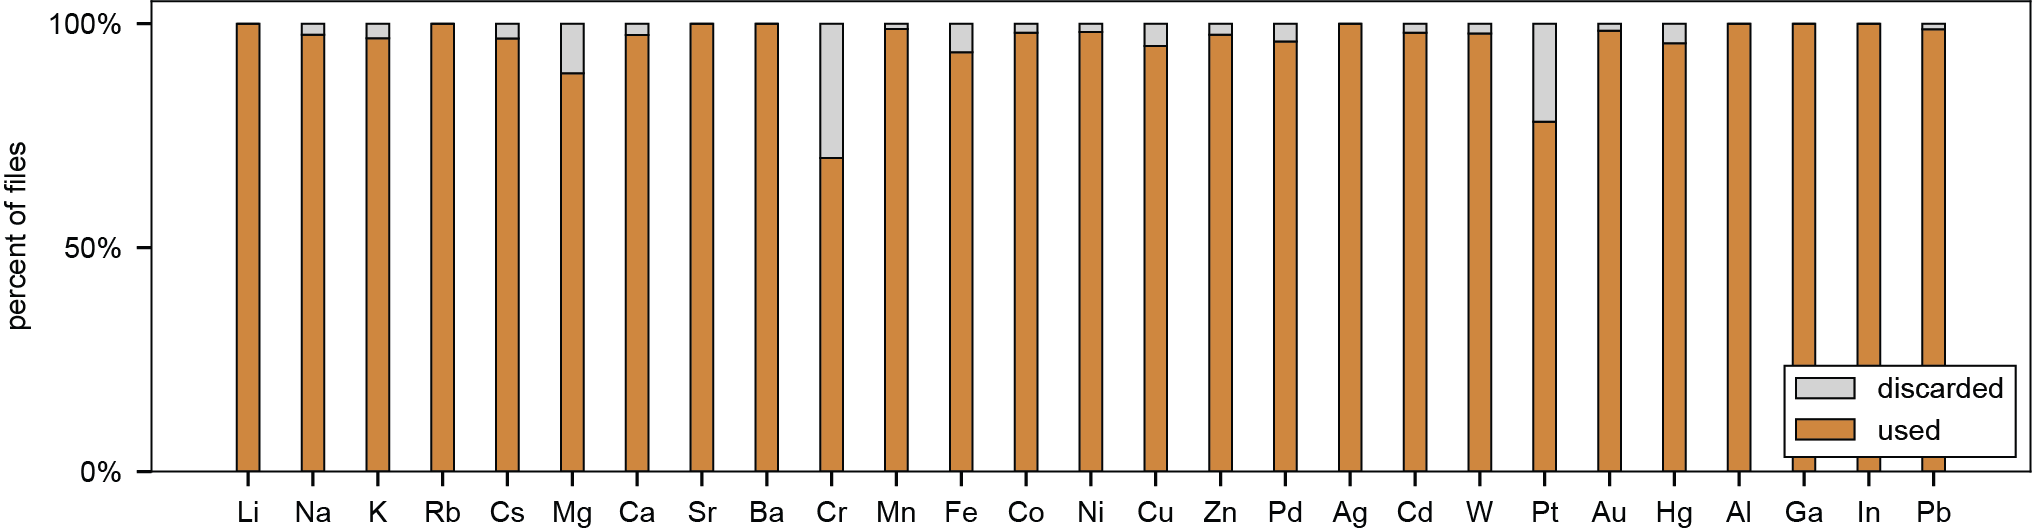
\includegraphics[width=\linewidth]{analysis-usable-files.png}
	\caption[Filtering metal PDB entries for incorrectly annotated or removed PDB entries]
	{
		\textbf{Filtering metal PDB entries for incorrectly annotated or removed PDB entries}.
		The chain letter and metal location were used to locate the metal center from the PDB entry. However, some annotations provided by the \mPDB{} were incorrect and led to wrongly assigned metal IDs or non-existent locations.
	}
	\label{\figname{C}{7}}
\end{figure}

Unfortunately, this additional step did eliminate more protein entries, as some of the annotations provided by the \mPDB{} were incorrect, or some protein structures were out of date (additional filtering step was discussed in \FIGURE~\ref{\figname{C}{2}}c,d). On average, approximately 2--10\% of files were discarded when attempting to retreive protein structures from the PDB using file information taken from the \mPDB{} (\FIGURE~\ref{\figname{C}{7}}).

%==============================%
% simplified schematic and data
%==============================%
\begin{figure}[H]
	\centering
	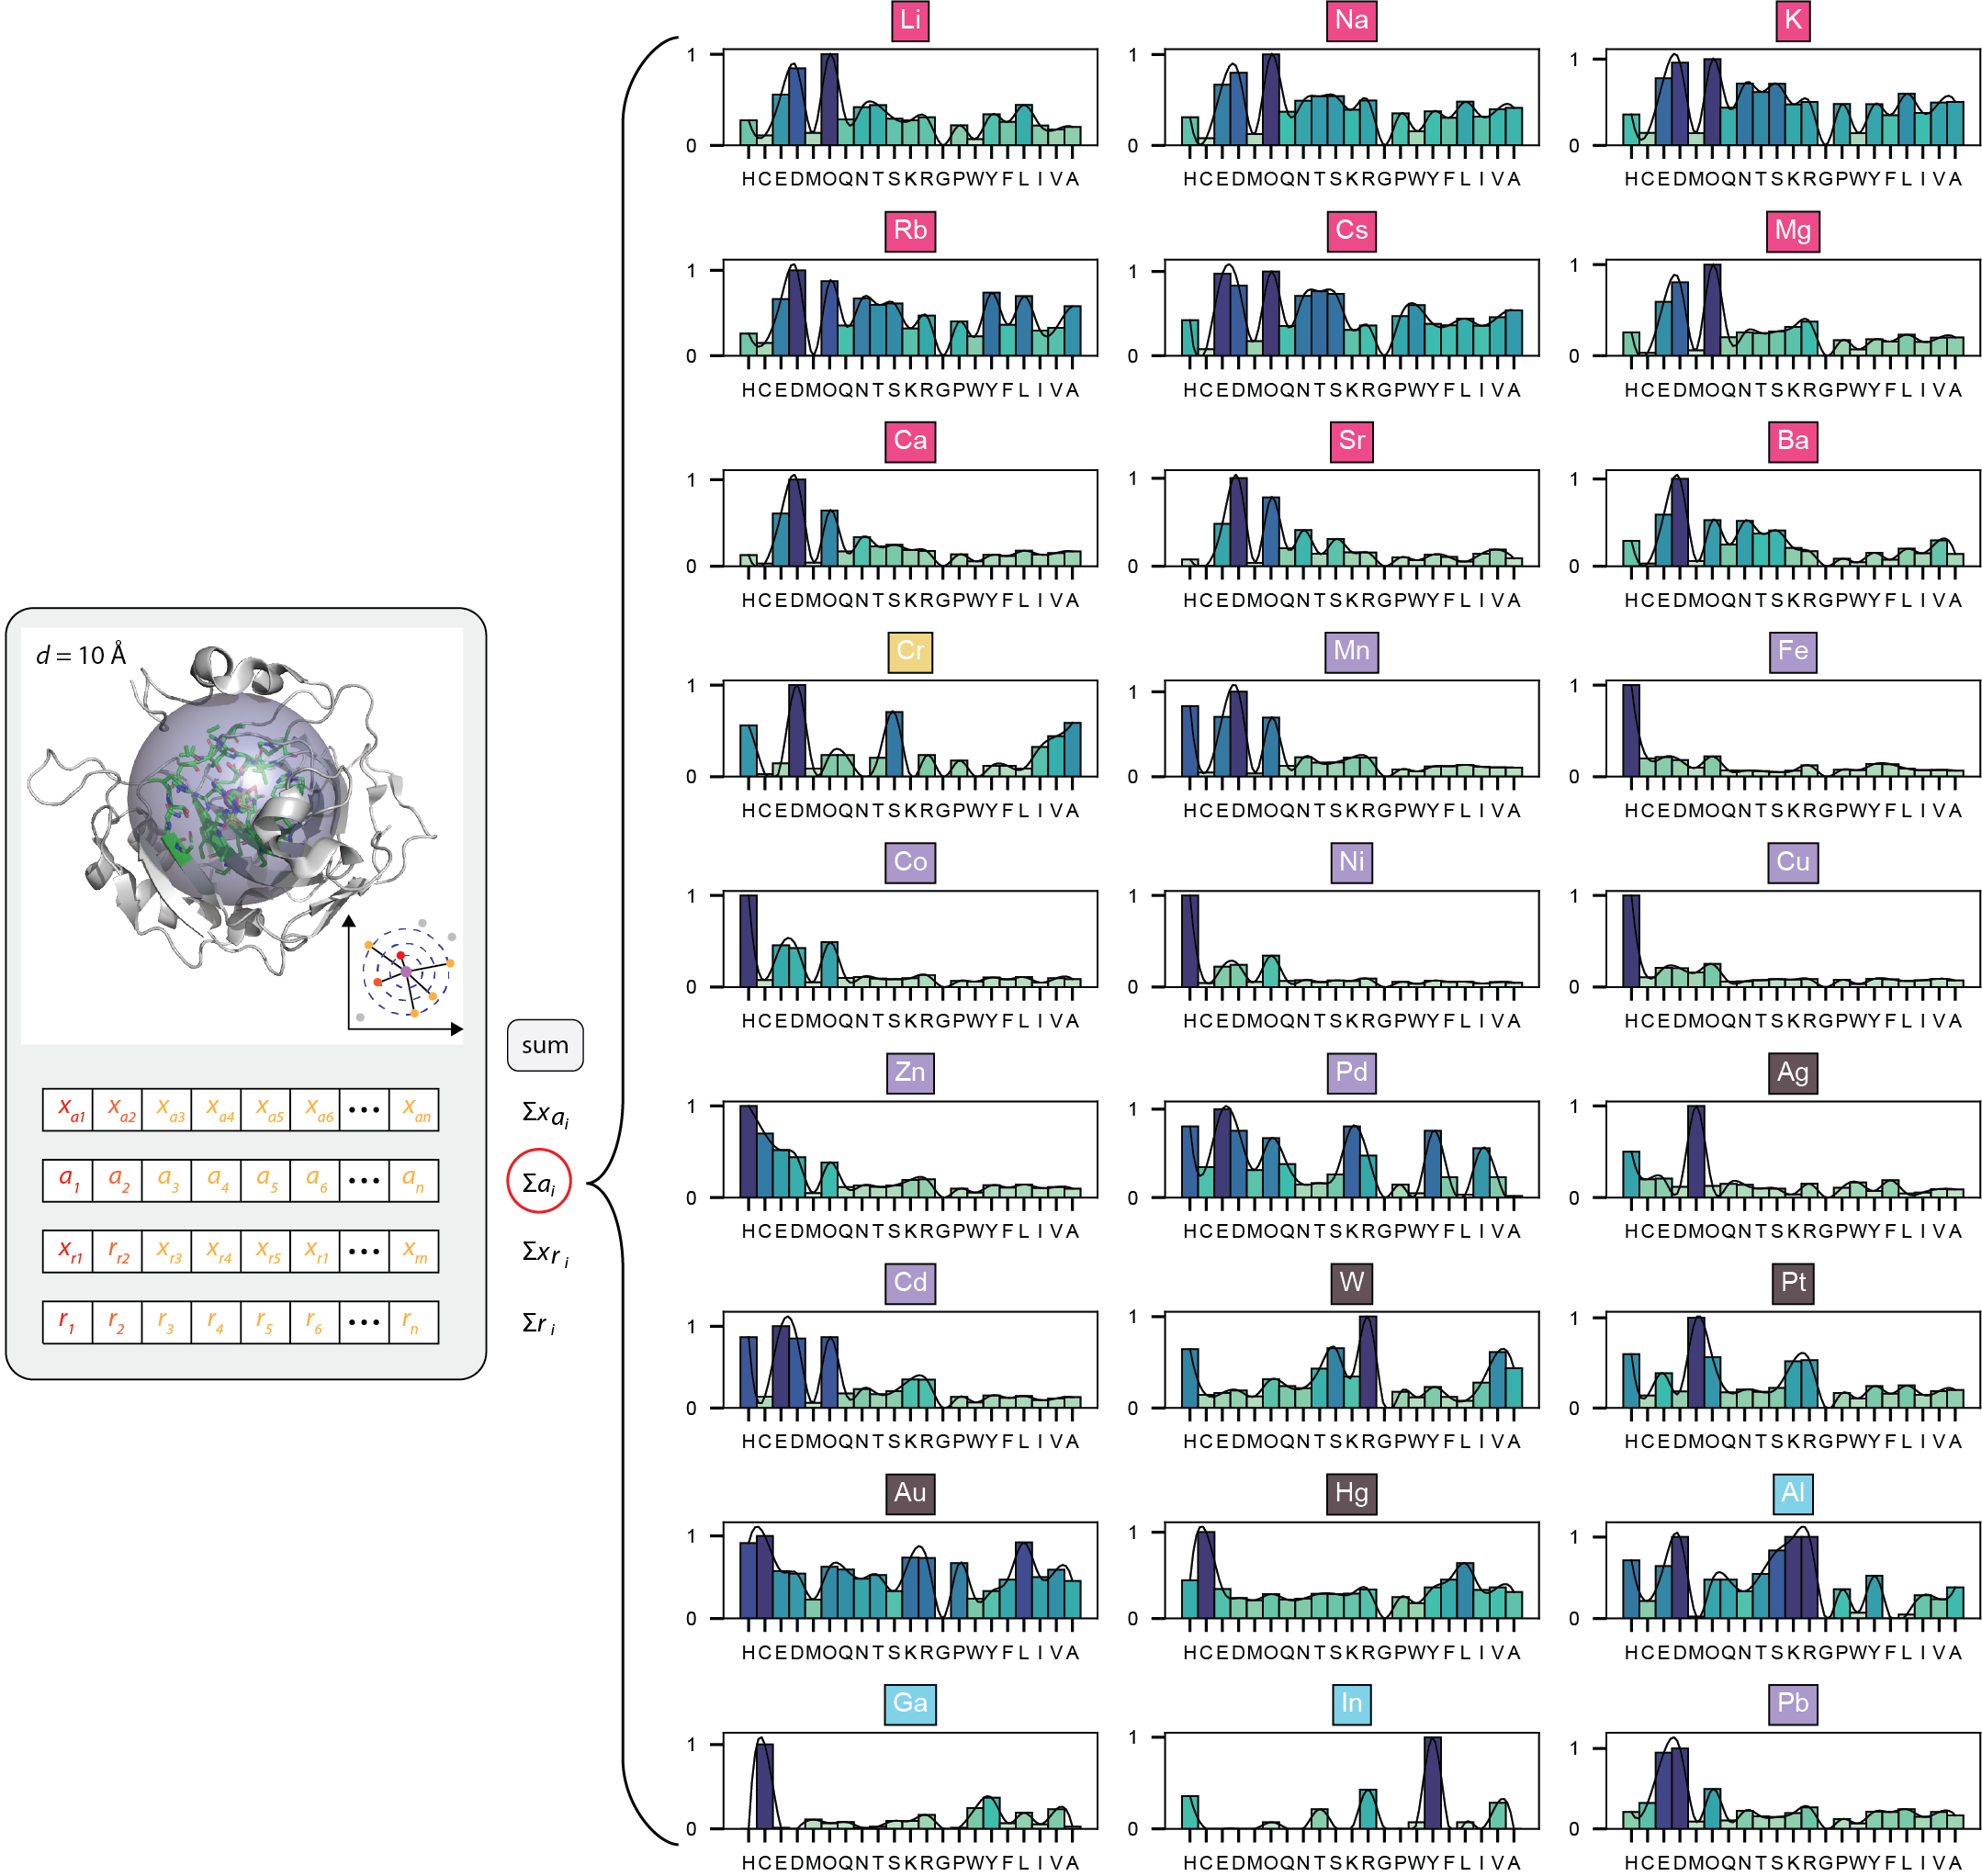
\includegraphics[width=\linewidth]{indepth-algorithm-residue-binning.png}
	\caption[Histogram of binned residue counts at 10 \AA away from the metal center]
	{
		\textbf{Histogram of binned residue counts at 10 \AA away from the metal center}.
		The frequency of occurance of residues encountered 10 \AA{} away from the metal center. The frequency plot represents a ``residue profile'' of the most common amino acids present in the vicinity of the metal-binding environment. Metal coloring for each plot title corresponds to the cluster they belong to, analyzed in \FIGURE~\ref{\figname{C}{11}}
	}
	\label{\figname{C}{8}}
\end{figure}

From the usable files, the metal center of each PDB entry was located, and the nearest-neighbors were tabulated for a given radii away from the metal. At each radii, an array was constructed by tabulating the nearest atom, distance, and the same for residues and their distances away from the metal (the data structure format was shown in \TABLE~\ref{\inputtable{C}{3}}). 

%====================%
% residue distribution
%====================%
\clearpage % clear page so they all fit (with caption included)
\begin{figure}[H]
	\begin{subfigure}[h]{\textwidth}
		\centering
		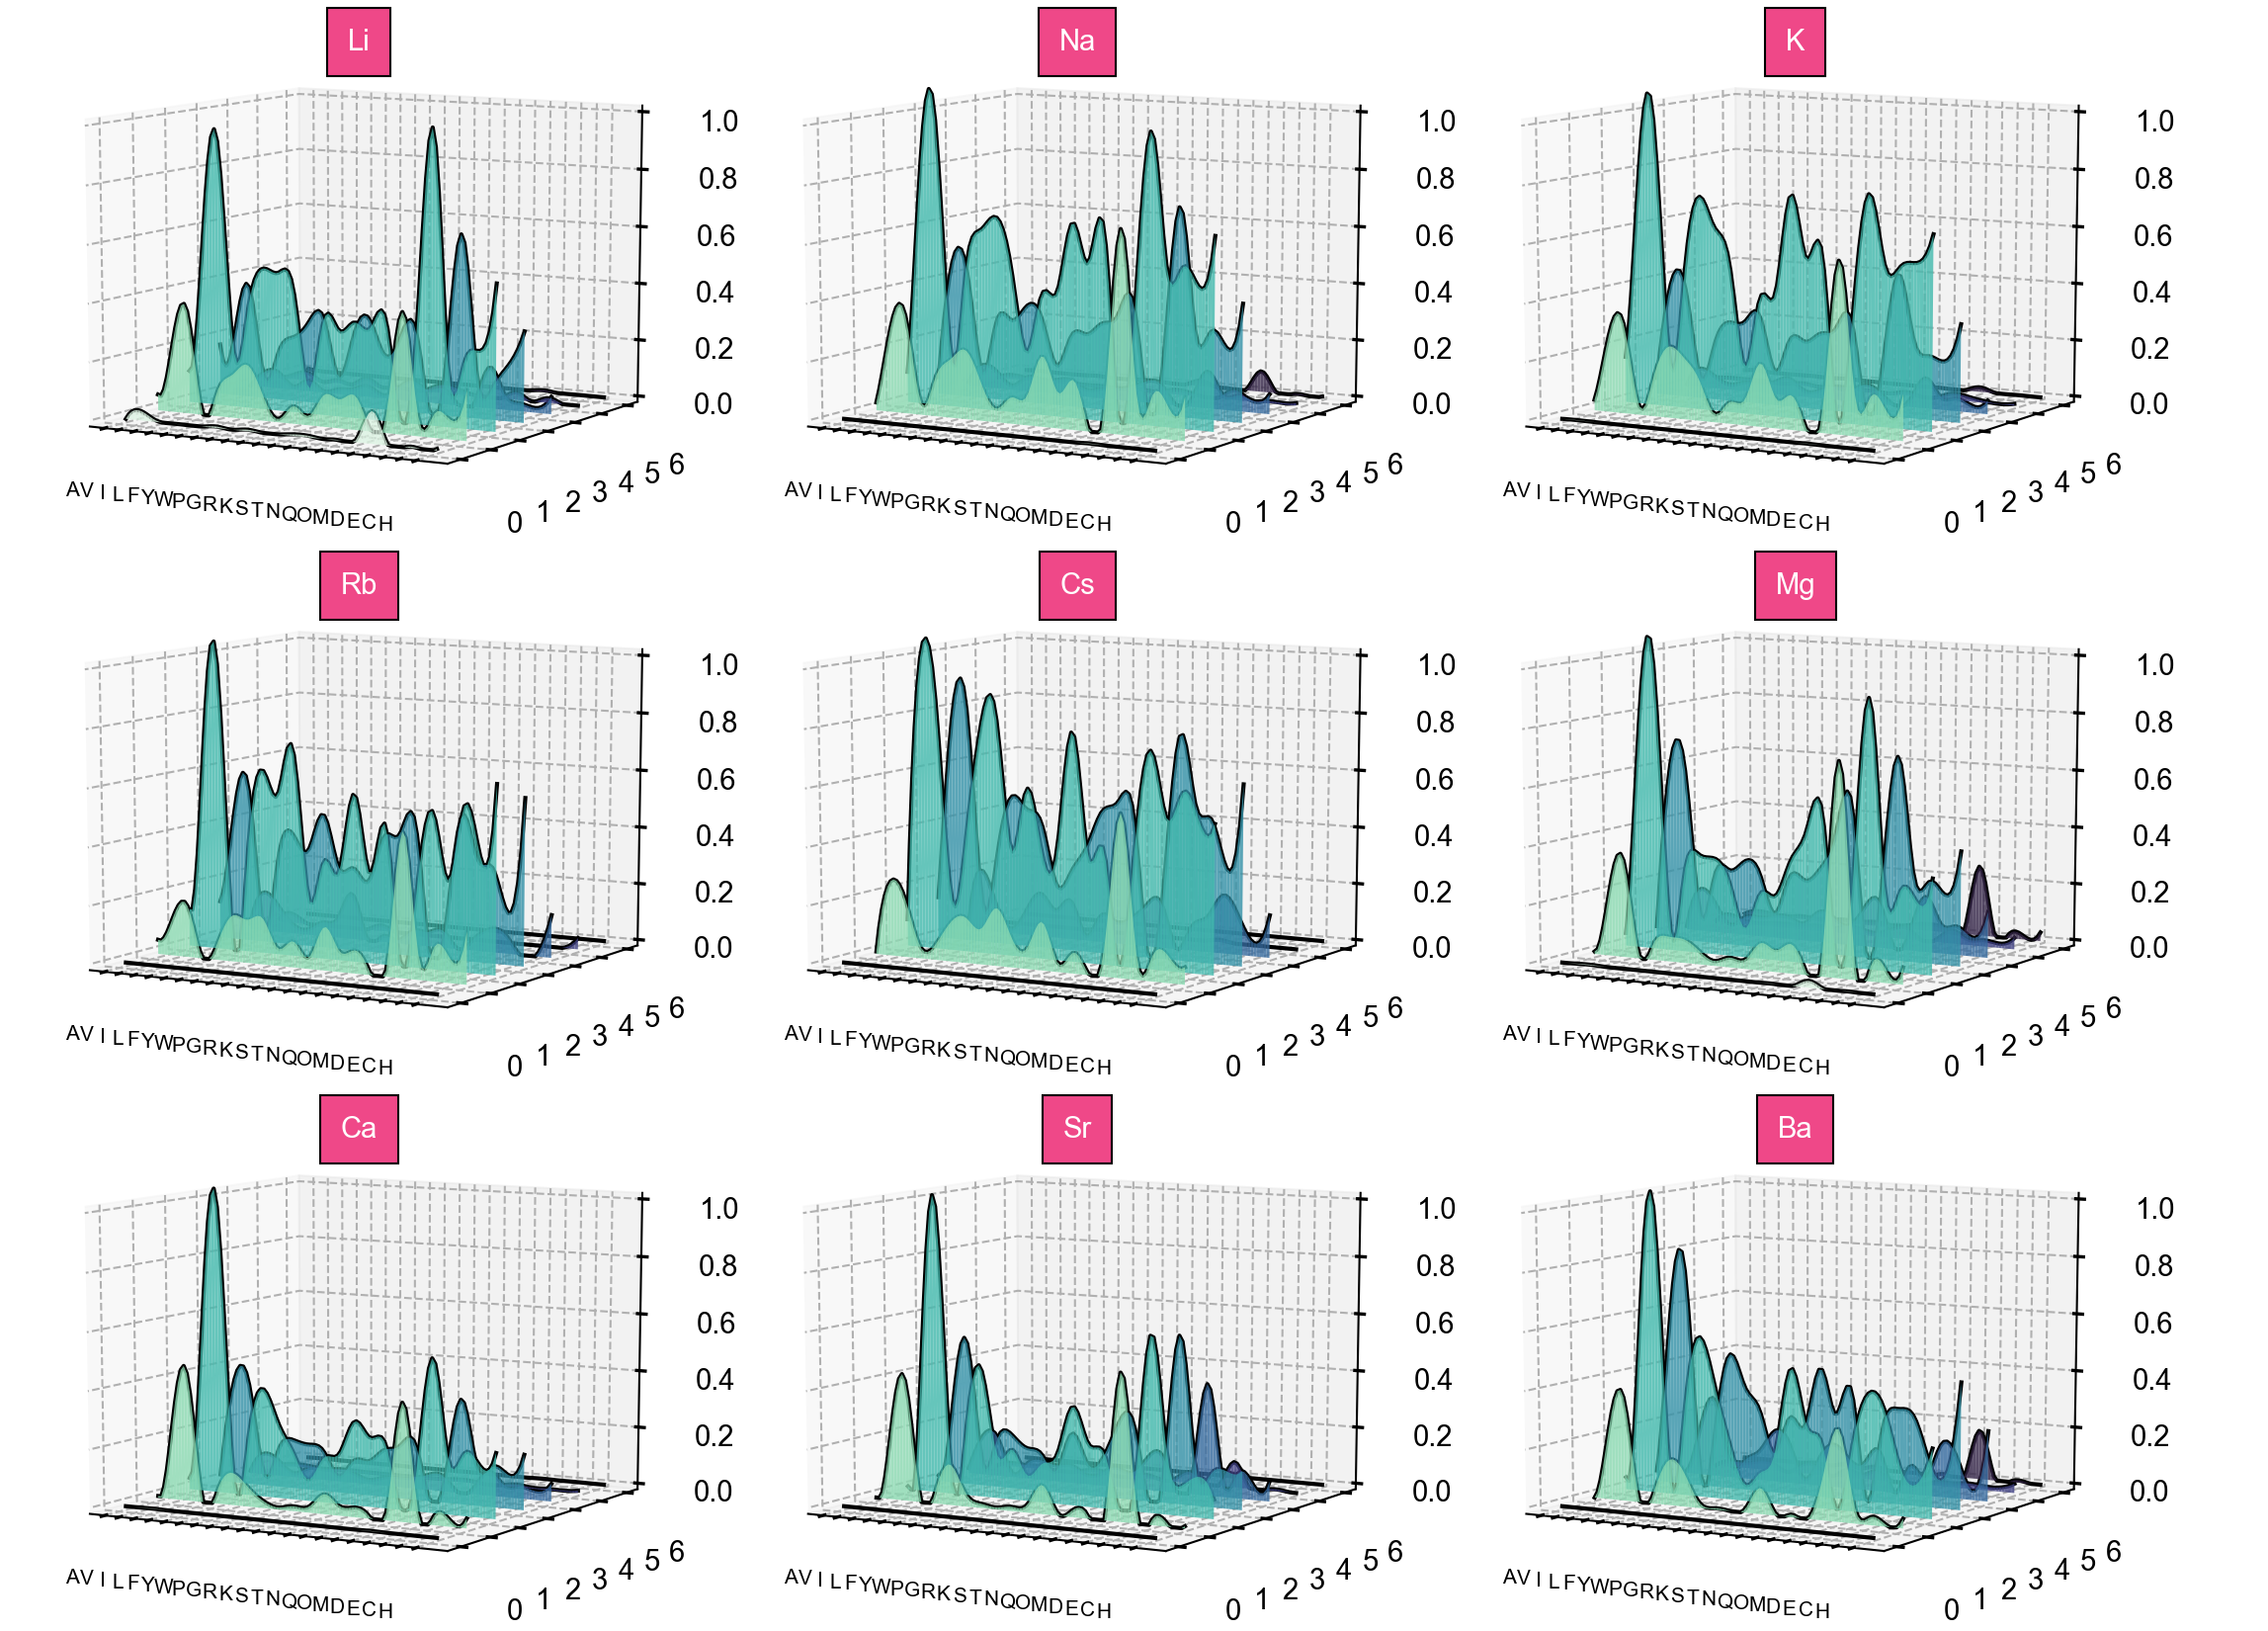
\includegraphics[height=0.4\paperheight]{analysis-subset-1.png}
	\end{subfigure}
\end{figure}
%
\vspace{-2\baselineskip}
%
\begin{figure}[H]\ContinuedFloat
	\begin{subfigure}[h]{\textwidth}
		\centering
		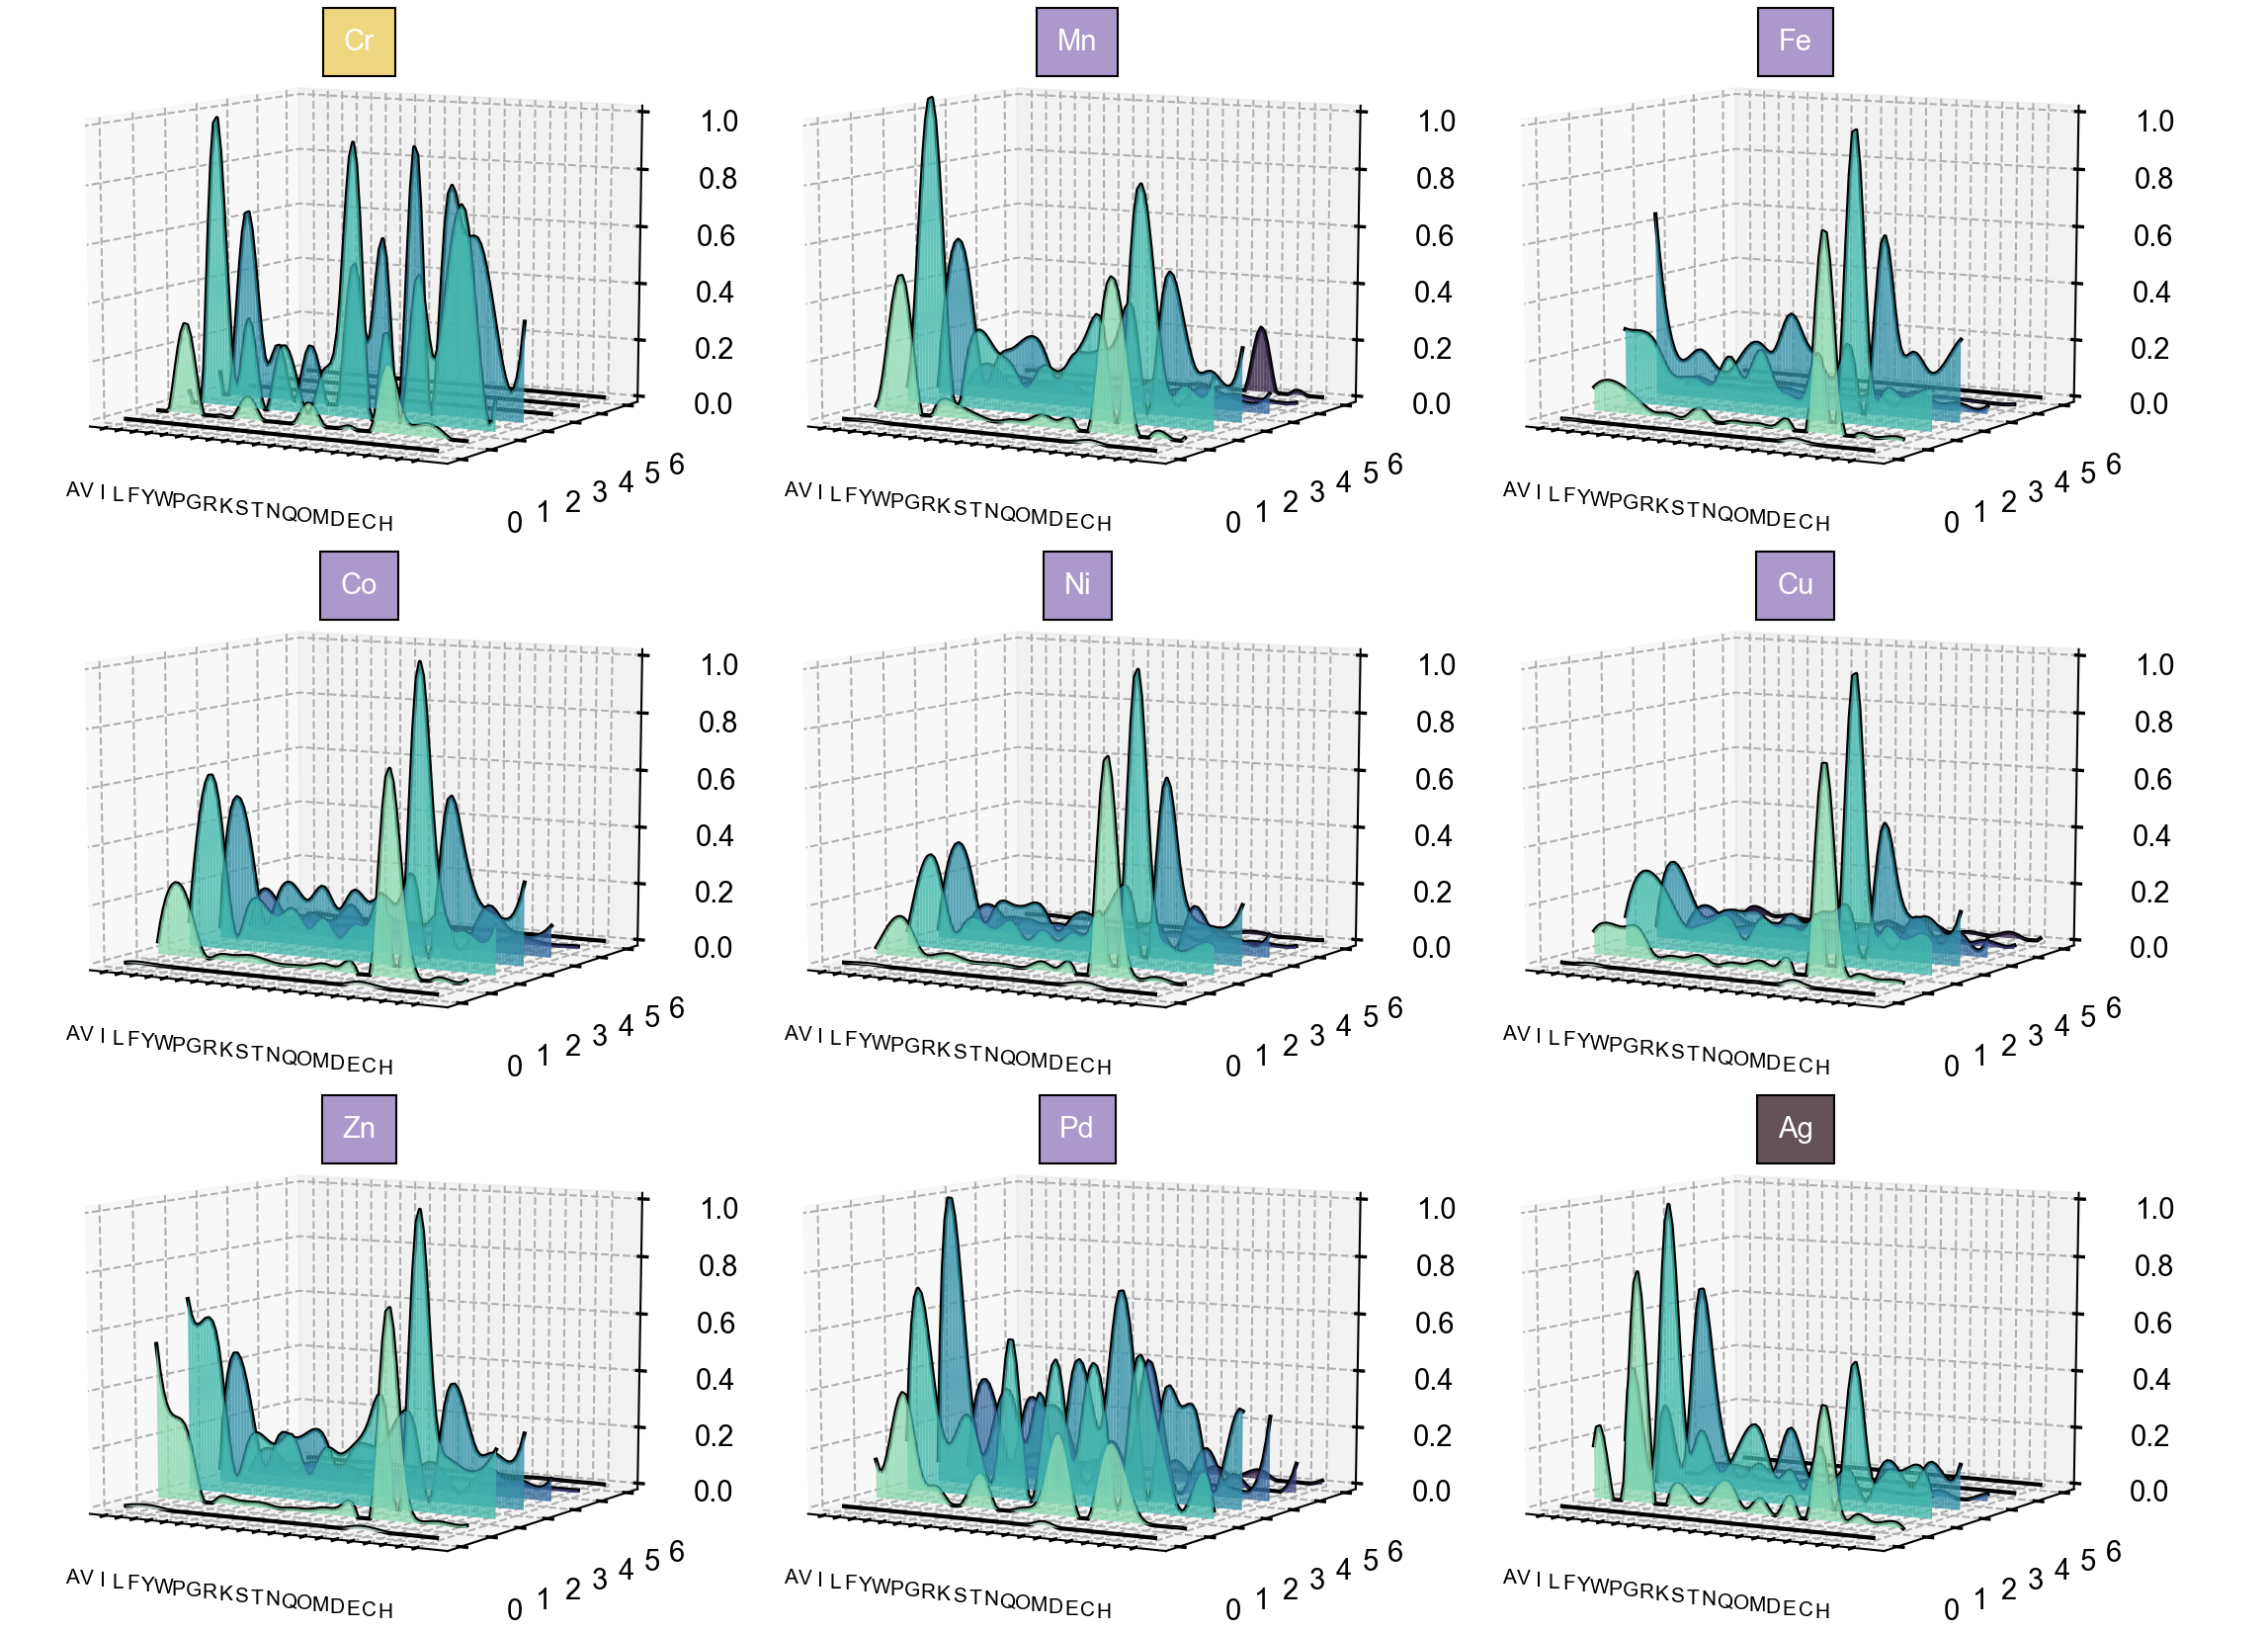
\includegraphics[height=0.4\paperheight]{analysis-subset-2.png}
	\end{subfigure}
\end{figure}
%
\vspace{-2\baselineskip}
%
\begin{figure}[H]\ContinuedFloat
	\begin{subfigure}[h]{\textwidth}
		\centering
		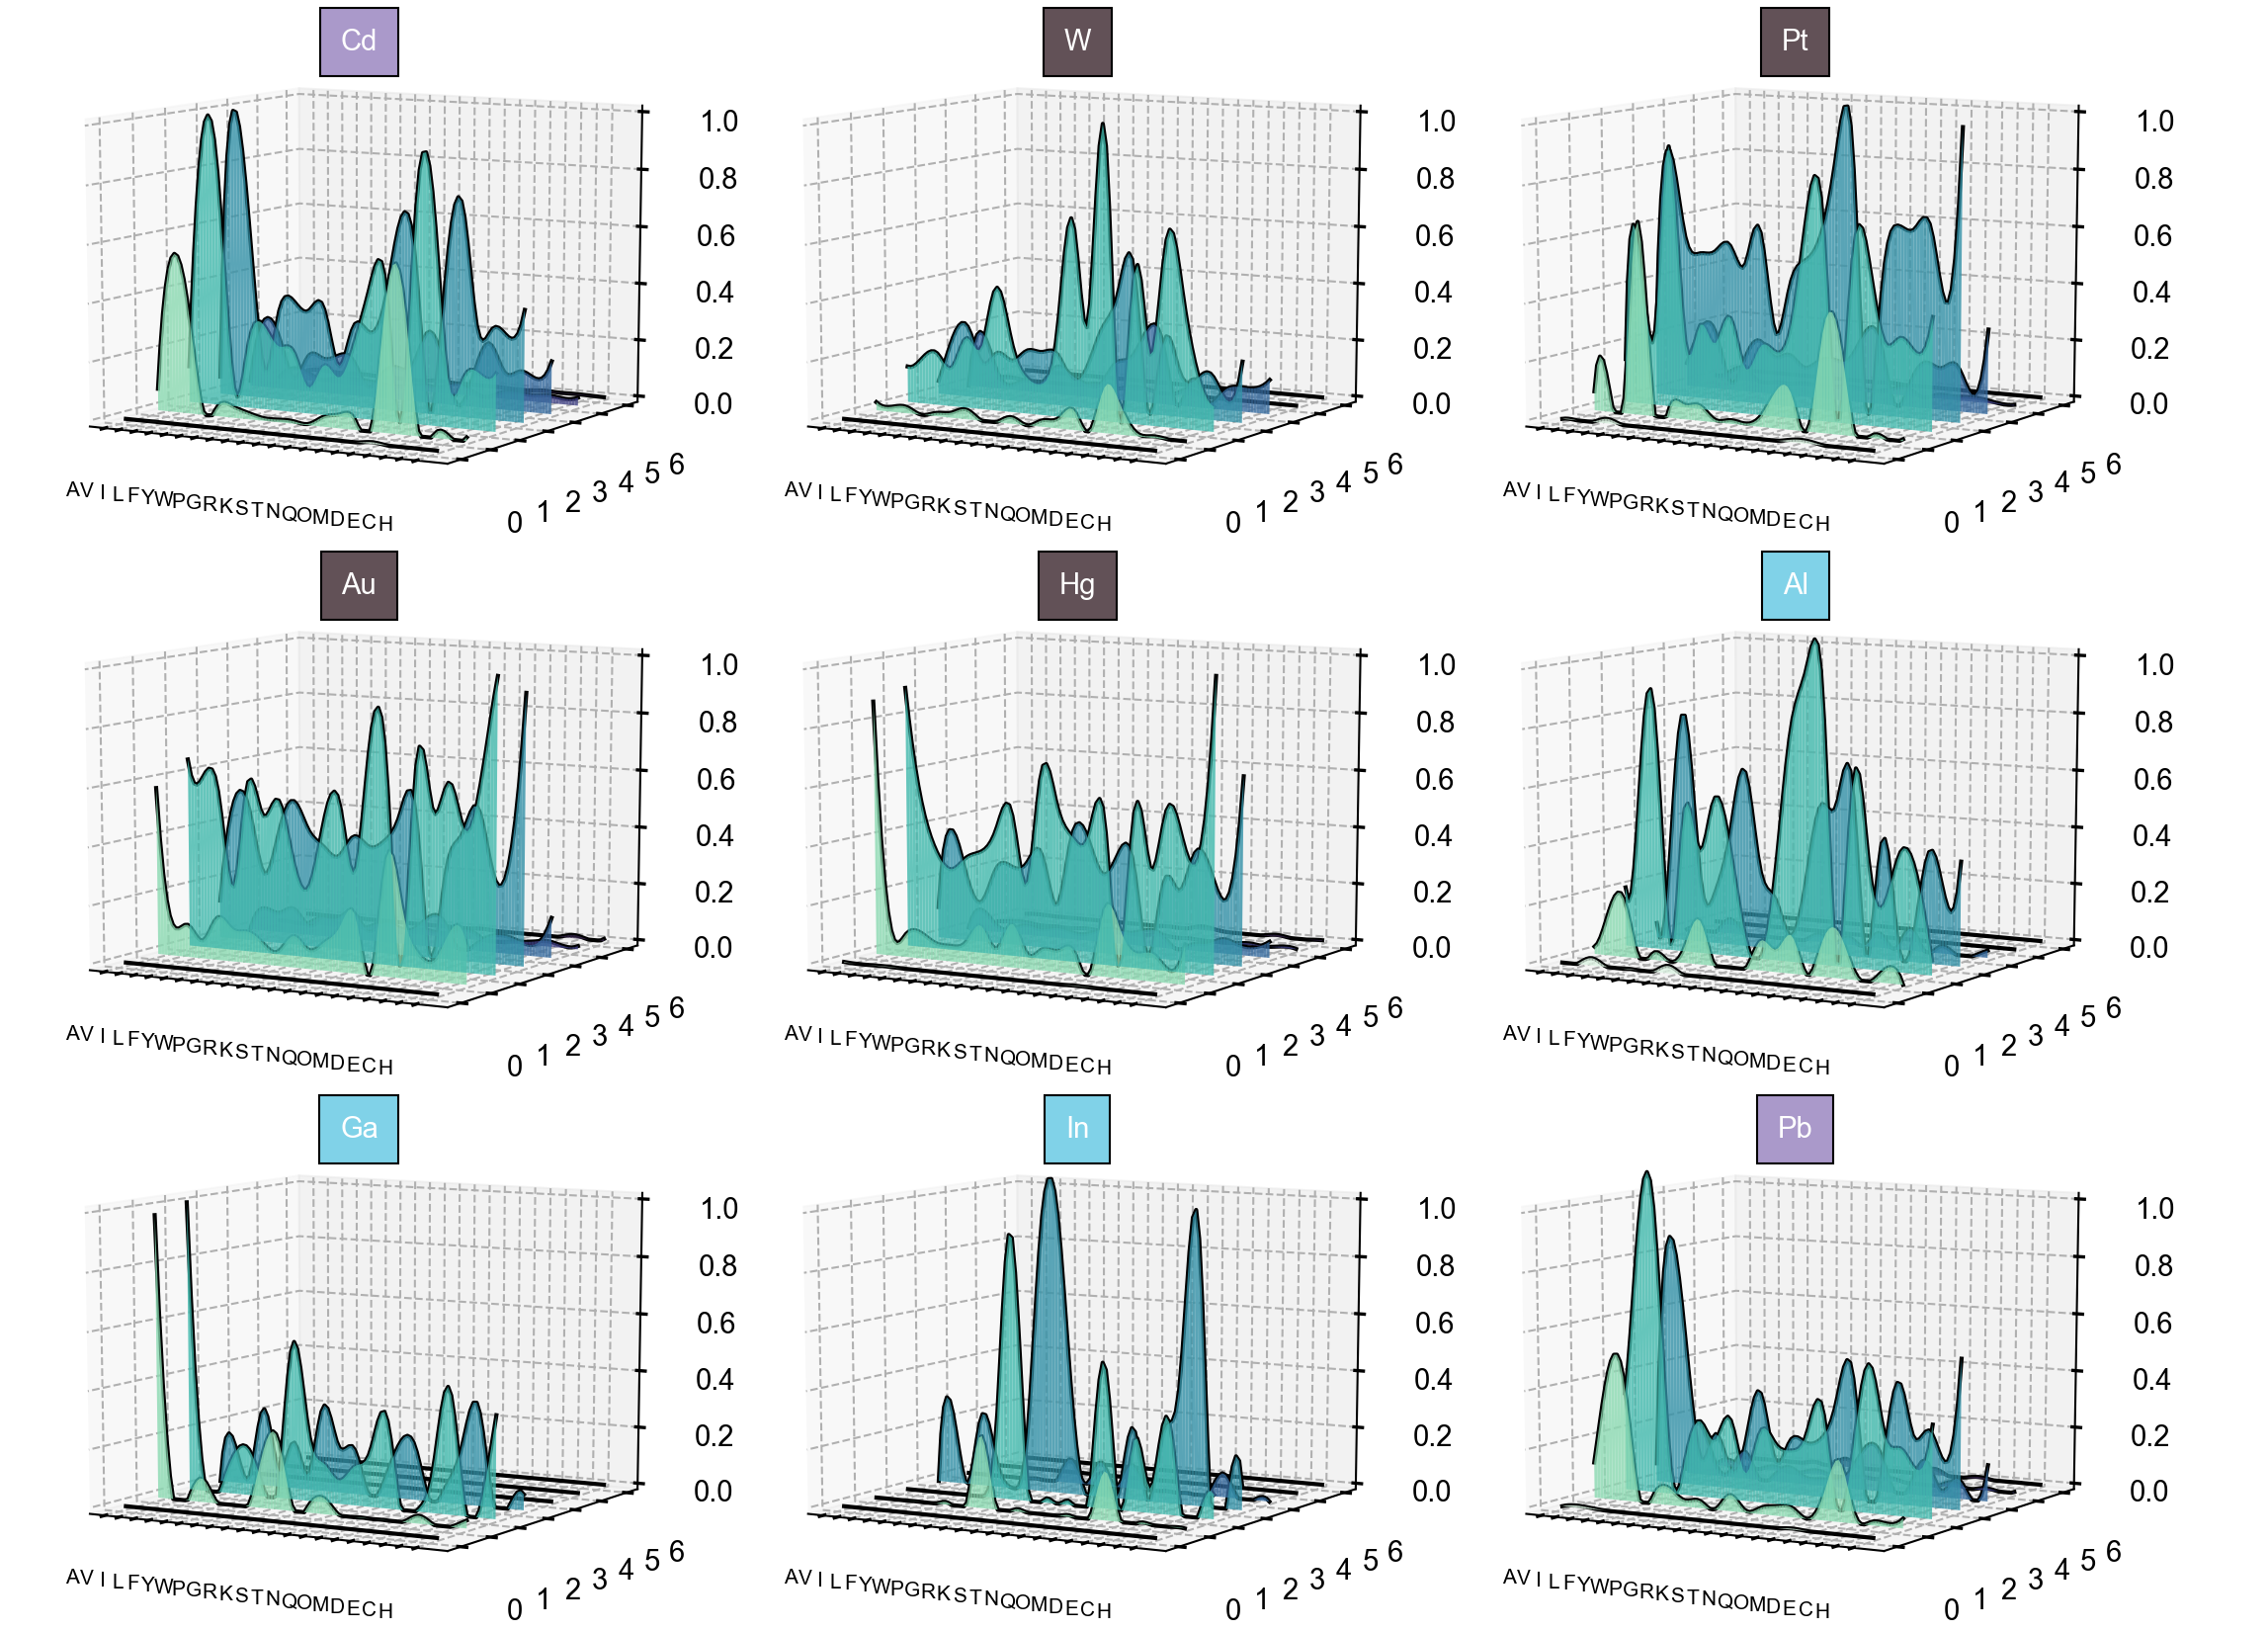
\includegraphics[height=0.4\paperheight]{analysis-subset-3.png}
	\end{subfigure}
	\caption[3-dimensional histogram of residue counts as a function of distance away from the metal center]
	{
		\textbf{3-dimensional histogram of residue counts as a function of distance away from the metal center}.
		x-axis (left most axis) are single code-letterings of amino acids. y-axis (right most axis) represent the distance in \AA{} away from the metal center. z-axis (vertical axis) represent the percent occurance of the amino acids at the given distance away, noramlized to 1.
	}
	\label{\figname{C}{9}}
\end{figure}


\noindent Each row represents a particular metal-protein interaction, and features were concatenations of atoms, residues, and their distances (in ascending order) away from the metal. Similar to counting the representation of ligands annotated by the \mPDB{}, the occurances of residues were counted and binned at each radii to create stacks of 2-dimensional histograms (\FIGURE~\ref{\figname{C}{8}}). These histograms represent a `residue profile', in other words the statistical representation of residues encountered as one moves away from the metal center.

Histograms of each radii slice can be stacked together to generate a 3-dimensional plot of residues encountered (x-axis) versus distance (y-axis) versus frequency of encountered residue (z-axis) (\FIGURE~\ref{\figname{C}{9}}).

Similarly, these same plots can be flattened to 2-dimensions by color encoding the z-axis as a heatmap (\FIGURE~\ref{\figname{C}{10}}).

%=====================%
% heatmap distribution
%=====================%
\begin{figure}[H]
	\centering
	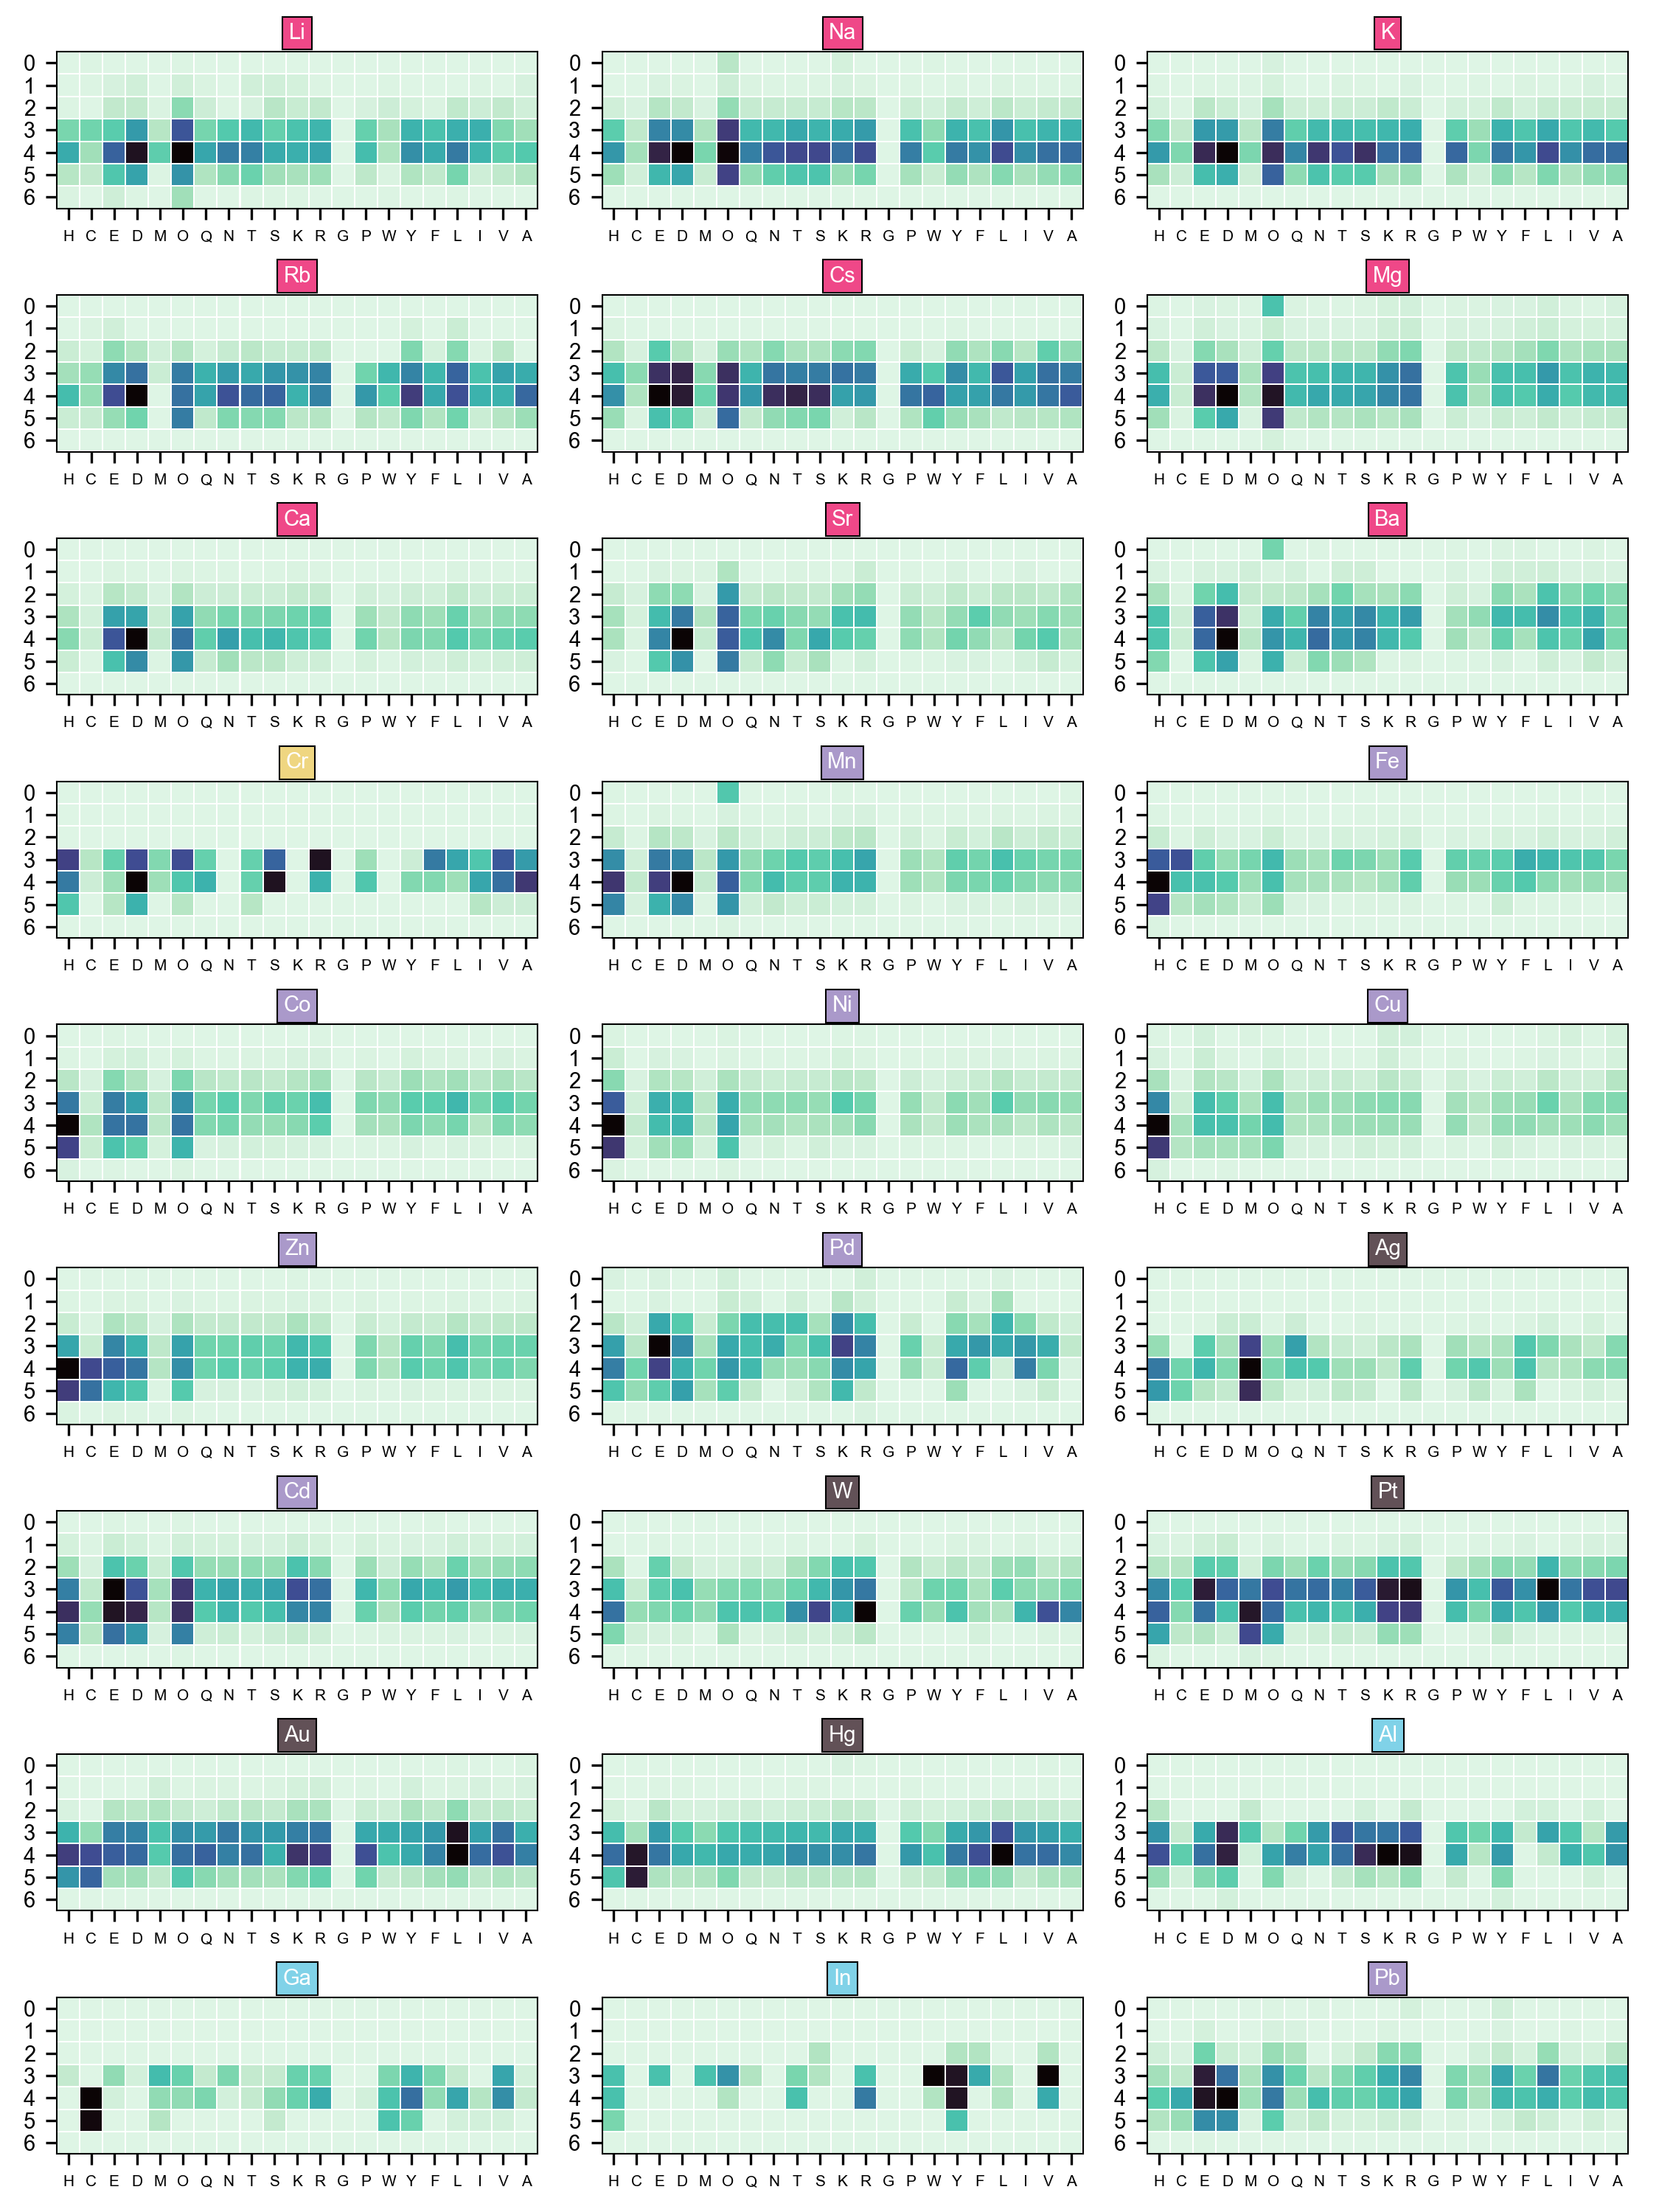
\includegraphics[width=\linewidth]{analysis-flat-heatmap.png}
	\caption[2-dimensional heatmap of residue counts as a function of distance away from the metal center]
	{
		\textbf{2-dimensional heatmap of residue counts as a function of distance away from the metal center}
	}
	\label{\figname{C}{10}}
\end{figure}

The 2-dimensional dataset for each metal can be further flattened to a 1-dimensional array with each row concatenated into a single vector.

%=====================%
% redo clustering
%=====================%
\begin{figure}[H]
	\centering
	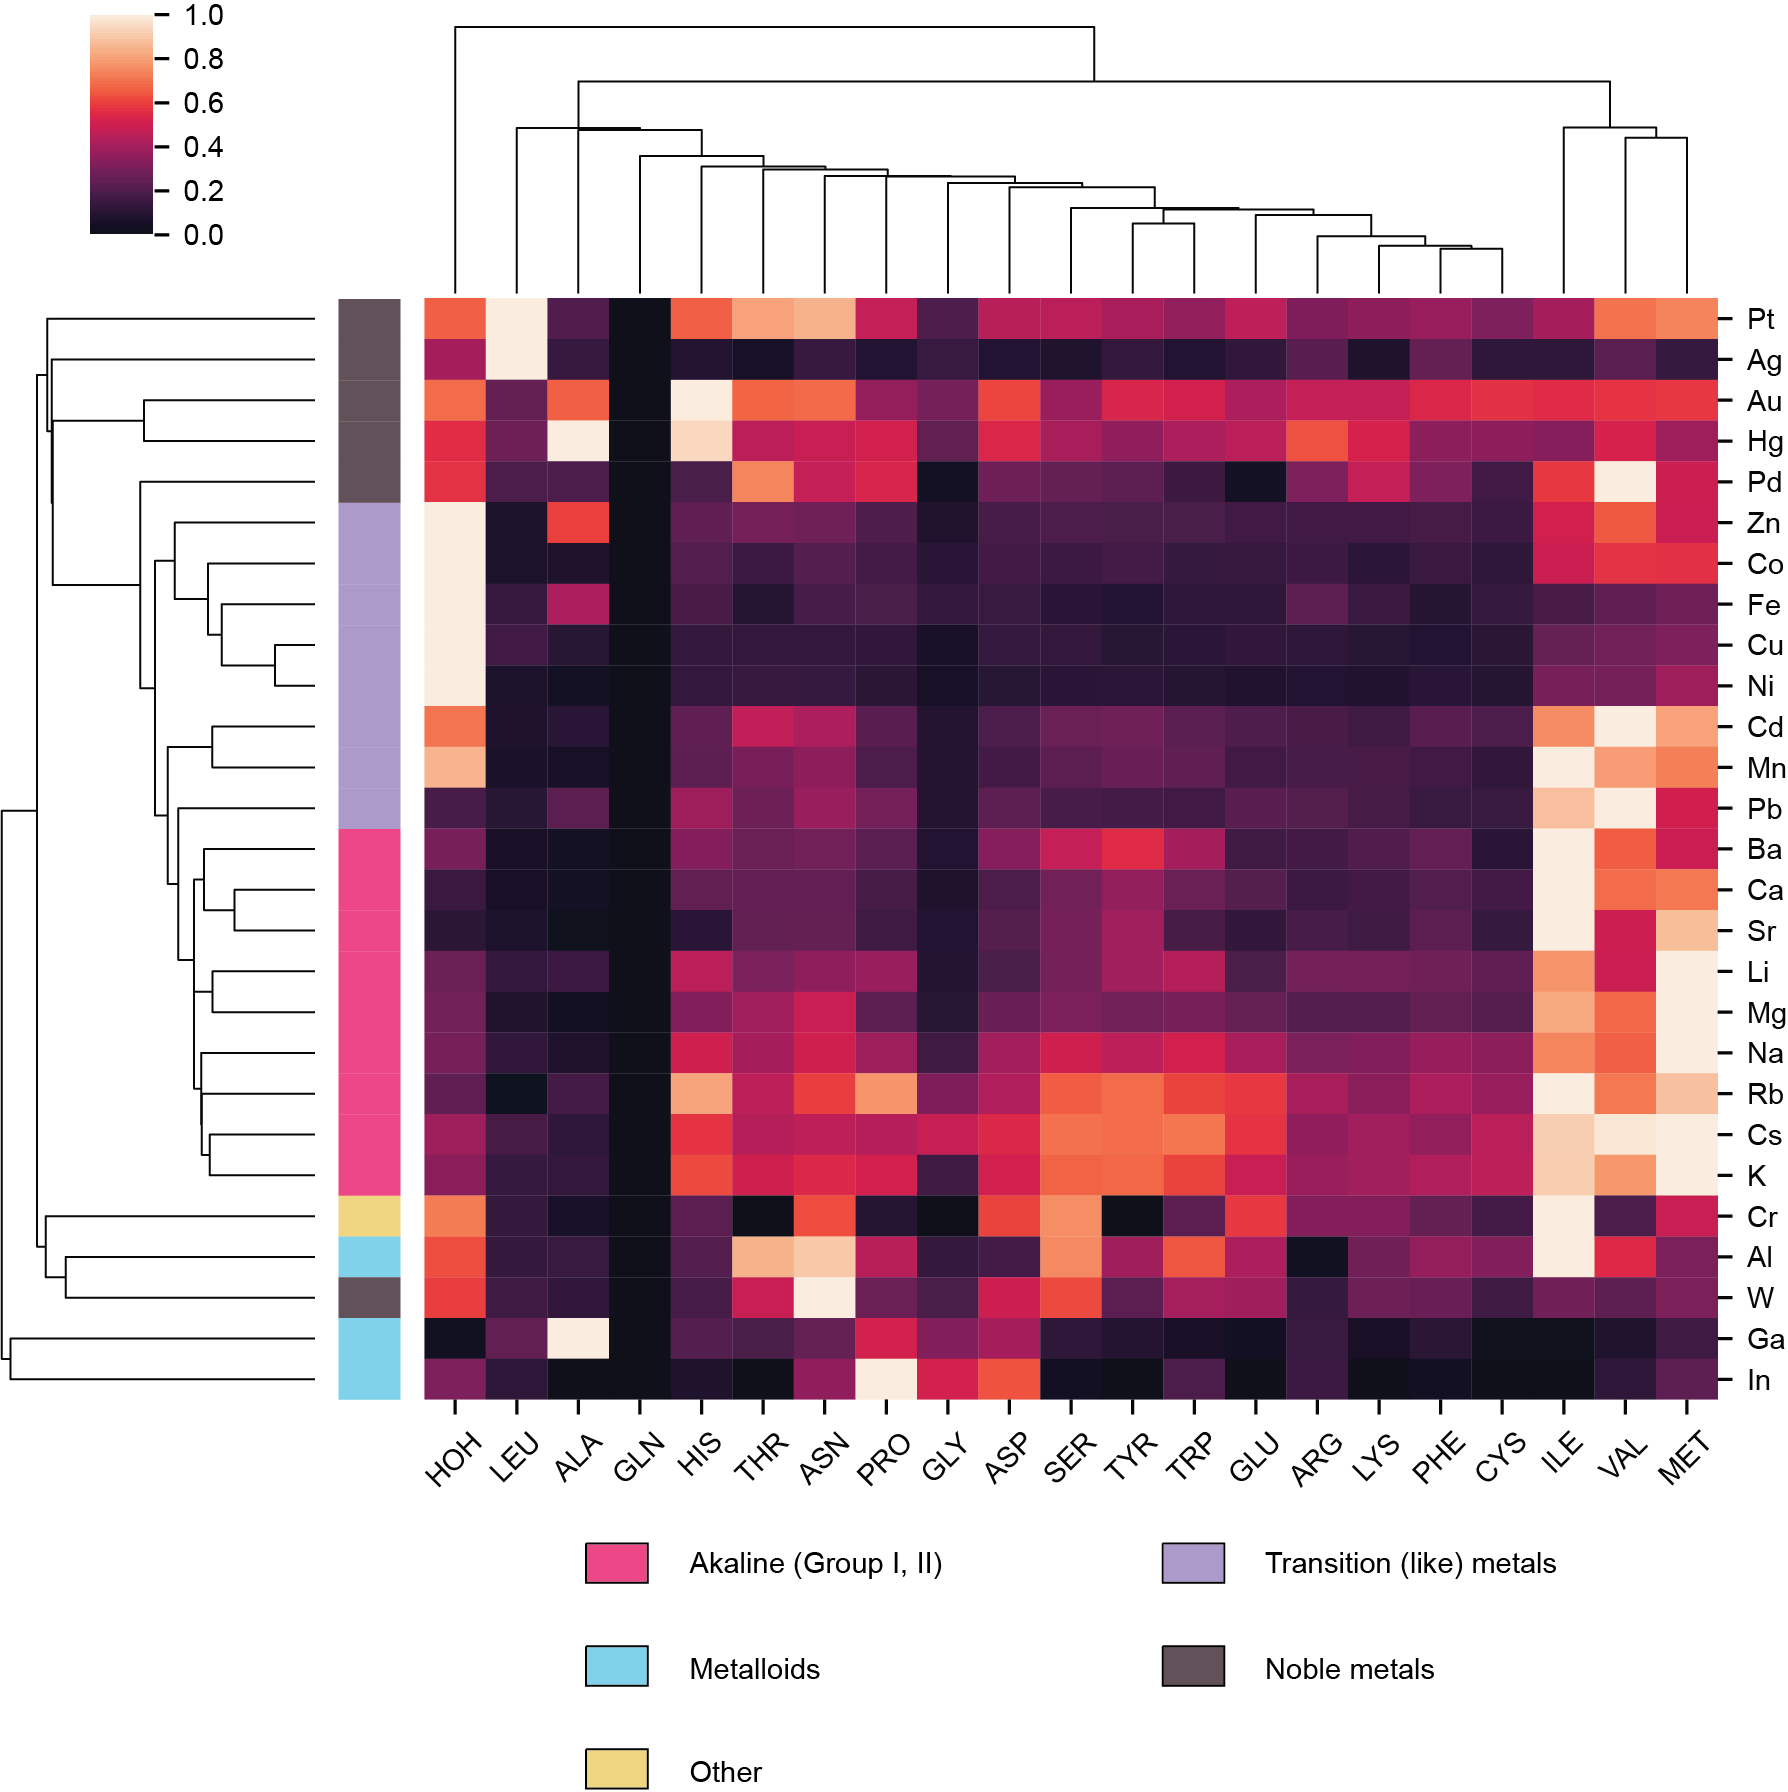
\includegraphics[width=\linewidth]{analysis-clustering.png}
	\caption[Improved metal clustering using new datasets derived from the modified nearest-neighbor algorithm]
	{
		\textbf{Improved metal clustering using new datasets derived from the modified nearest-neighbor algorithm}.
		Data on amino acid occurances as a function of distance away from the metal center provided a more data rich analysis compared to data provided from the \mPDB{} (\FIGURE~\ref{\figname{C}{6}}). In addition, the segregation of metal groups was more distinct, as each periodic grouping: alkaline/alkaline-earth metals (pink rows), transition metals (light purple rows), noble metals (brown rows), and metalloids (turquoise rows), were segregated from one another with statistical significance. The only outliers were W (tungsten), which grouped into the metalloid cluster, and Cr (chromium), which was distinguished as its own group.
	}
	\label{\figname{C}{11}}
\end{figure}

\noindent With this, the same clustering analysis performed for \FIGURE~\ref{\figname{C}{6}} could be done. The result is an improved segregation of metal groups given the more feature rich dataset (\FIGURE~\ref{\figname{C}{11}}).

%===========================================================================%
% SECTION
%===========================================================================%
\section{Statistical analysis and machine learning; future work}
Future work needs to be done to further investigate different feature extraction strategies and appropriate usage of statistical and machine learning models. This work is under current investigation and is under active research. The goal of this future work is to take the insights from the previous sections and machine learning models for predicitve or generative purposes. Examples include predicting the metal identity in unknown metal-binding pockets, or generating de-novo protein-metal binding environments.

\noindent Future steps to take include:

\begin{itemize}
	\item \textbf{Further feature extraction and engineering} \\
	Only residue counts as a function of distance were used as features for the clustering analysis (\FIGURE~\ref{\figname{C}{11}}). Yet there are many features not used, such as the distance between metal and residues, and the same for the nearest atoms. Other features can be calculated such as the euclidean angle between metal and residues, or trigonometric parameters between residues in the same binding sphere. More sophisticated 3-dimensional analytics can be performed to solve for the sphere of hydration between the metal and resiudes, or the accessible surface topology of the metal binding pocket. In addition, metadata such as $\beta$-factor, percent occupancy, and other intrinsic data to the PDB structure can be used to weigh specific entries such that outliers are supressed during analysis.
	%
	\item \textbf{Dimensionality reduction} \\
	Too many features add noise or unnecessarily increase computational time. In most cases too many features may contribute to overfitting. Therefore, dimensional reduction techniques such as principal component analysis should be used to determine the most fundamental linear combinations of features that still fully represent the dataset. Dimensionality reduction can also project the dataset onto another plane that better discriminates instances; for example, projecting a cone from the top to form can separate the heights of the cone on a 2-dimensional plane. However, a poor projection from the side would overlap the surfaces of the cone into a triangle. So testing a variety of dimensional reduction techniques should be checked before proceeding to training machine models .
	%
	\item \textbf{Experiments with a variety of classifier models} \\
	There exist numerous machine learning models, many with their own benefits and drawbacks. Each model should be tested empirically to determine which performs the best. For this purpose classifiers would be appropriate, as the model should be able to classify which arrangement of residues have the highest probability of containing a certain metal. Examples of classifiers are decision trees or random forrests.
	%
	\item \textbf{Hyperparameter tuning using gridsearch} \\
	Mostly all models do not work ``out of the box'' and need fine tuning to adjust for the nuances of a particular dataset. These parameters, such as rate of learning, variable weights, and so on, are called hyperparameters. Often, these hyperparameters are brute-forced optimized through grid searching, where several hyperparameters are permutated for a single training run, and performed repeatedly over the entire combinatorial space of hyperparameters until a value is selected that optimizes the training output, or reduces the error.
	%
	\item \textbf{Creating pipelines for ensemble learning} \\
	Several algorithms can work in conjunction to provide better modeling and decision power. Examples include large or convulational neural networks, algorithms sub-classified as deep learning algorithms. With these new algorithms, the pipeline of feature engineering, dimensionality reduction, and hyperparameter tuning may need to be further optimized.
\end{itemize}

One overaching concern is whether the quantity and quality of PDB entries is enough to robustly train a model to accurately predict metal-binding interactions. So far there are 151,754 protein structures in the PDB\footnote{
	statistics on the PDB can be found here: \url{https://www.rcsb.org/stats}
}. However, some are redundant, and the quality varies dramatically between entires. It actually may be too early, or ambitious, to study every protein structure as the data is not yet sufficient to train a suitable machine model. Another setback may be the difficulty to extract useful features from a complex 3-dimensional crystal structure, and that algorithms have not yet been developed. However, the work so far suggest that it may be possible to cluster groups of similar metals together, and that may be enough to help create custom peptide/proteins with affinities for alkaline and alkaline-earth metal from the transition, noble, and metalloids.

%===============================BIBLIOGRAPHY================================%
\printbibliography[title=References]

\end{document}
